% A LaTeX template for ARTICLE version of the MSc Thesis submissions to 
% Politecnico di Milano (PoliMi) - School of Industrial and Information Engineering
%
% S. Bonetti, A. Gruttadauria, G. Mescolini, A. Zingaro
% e-mail: template-tesi-ingind@polimi.it
%
% Last Revision: October 2021
%
% Copyright 2021 Politecnico di Milano, Italy. Inc. NC-BY

\documentclass[11pt,a4paper]{article} 

%------------------------------------------------------------------------------
%	REQUIRED PACKAGES AND  CONFIGURATIONS
%------------------------------------------------------------------------------
% PACKAGES FOR TITLES
\usepackage{titlesec}
\usepackage{color}

% PACKAGES FOR LANGUAGE AND FONT
\usepackage[utf8]{inputenc}
\usepackage[english]{babel}
\usepackage[T1]{fontenc} % Font encoding

% PACKAGES FOR IMAGES
\usepackage{graphicx}
\graphicspath{{Images/}}
\usepackage{eso-pic} % For the background picture on the title page
\usepackage{subfig} % Numbered and caption subfigures using \subfloat
\usepackage{caption} % Coloured captions
\usepackage{transparent}
\usepackage{tikz}
\usetikzlibrary{angles}

% STANDARD MATH PACKAGES
\usepackage{amsmath}
\usepackage{amsthm}
\usepackage{amsfonts}
\usepackage{bm}
\usepackage[overload]{empheq}  % For braced-style systems of equations

% PACKAGES FOR TABLES
\usepackage{tabularx}
\usepackage{longtable} % tables that can span several pages
\usepackage{colortbl}

% PACKAGES FOR ALGORITHMS (PSEUDO-CODE)
\usepackage{algorithm}
\usepackage{algorithmic}

% PACKAGES FOR REFERENCES & BIBLIOGRAPHY
\usepackage[colorlinks=true,linkcolor=black,anchorcolor=black,citecolor=black,filecolor=black,menucolor=black,runcolor=black,urlcolor=black]{hyperref} % Adds clickable links at references
\usepackage{cleveref}
\usepackage[square, numbers, sort&compress]{natbib} % Square brackets, citing references with numbers, citations sorted by appearance in the text and compressed
\bibliographystyle{plain} % You may use a different style adapted to your field

% PACKAGES FOR THE APPENDIX
\usepackage{appendix}

% PACKAGES FOR ITEMIZE & ENUMERATES 
\usepackage{enumitem}

% OTHER PACKAGES
\usepackage{amsthm,thmtools,xcolor} % Coloured "Theorem"
\usepackage{comment} % Comment part of code
\usepackage{fancyhdr} % Fancy headers and footers
\usepackage{lipsum} % Insert dummy text
\usepackage{tcolorbox} % Create coloured boxes (e.g. the one for the key-words)
\usepackage{listings}


%-------------------------------------------------------------------------
%	NEW COMMANDS DEFINED
%-------------------------------------------------------------------------
% EXAMPLES OF NEW COMMANDS -> here you see how to define new commands
\newcommand{\bea}{\begin{eqnarray}} % Shortcut for equation arrays
\newcommand{\eea}{\end{eqnarray}}
\newcommand{\e}[1]{\times 10^{#1}}  % Powers of 10 notation
\newcommand{\mathbbm}[1]{\text{\usefont{U}{bbm}{m}{n}#1}} % From mathbbm.sty
\newcommand{\pdev}[2]{\frac{\partial#1}{\partial#2}}
% NB: you can also override some existing commands with the keyword \renewcommand

%----------------------------------------------------------------------------
%	ADD YOUR PACKAGES (be careful of package interaction)
%----------------------------------------------------------------------------


%----------------------------------------------------------------------------
%	ADD YOUR DEFINITIONS AND COMMANDS (be careful of existing commands)
%----------------------------------------------------------------------------


% Do not change Configuration_files/config.tex file unless you really know what you are doing. 
% This file ends the configuration procedures (e.g. customizing commands, definition of new commands)
% Configuration package
\usepackage[bottom=2.0cm,top=2.0cm,left=2.0cm,right=2.0cm]{geometry}
\raggedbottom 

% Create color bluePoli (-> manuale grafica coordinata:  https://www.polimi.it/fileadmin/user_upload/il_Politecnico/grafica-coordinata/2015_05_11_46xy_manuale_grafica_coordinata.pdf)
\definecolor{bluePoli}{cmyk}{0.4,0.1,0,0.4}

% Custom theorem environments
\declaretheoremstyle[
  headfont=\color{bluePoli}\normalfont\bfseries,
  bodyfont=\color{black}\normalfont\itshape,
]{colored}

\captionsetup[figure]{labelfont={color=bluePoli}} % Set colour of the captions
\captionsetup[table]{labelfont={color=bluePoli}} % Set colour of the captions
\captionsetup[algorithm]{labelfont={color=bluePoli}} % Set colour of the captions

\theoremstyle{colored}
\newtheorem{theorem}{Theorem}[section]
\newtheorem{proposition}{Proposition}[section]

% Enhances the features of the standard "table" and "tabular" environments.
\newcommand\T{\rule{0pt}{2.6ex}}
\newcommand\B{\rule[-1.2ex]{0pt}{0pt}}

% Algorithm description
\newcounter{algsubstate}
\renewcommand{\thealgsubstate}{\alph{algsubstate}}
\newenvironment{algsubstates}{
    \setcounter{algsubstate}{0}%
    \renewcommand{\STATE}{%
    \stepcounter{algsubstate}%
    \Statex {\small\thealgsubstate:}\space}
    }{}
    
% Custom theorem environment
\newcolumntype{L}[1]{>{\raggedright\let\newline\\\arraybackslash\hspace{0pt}}m{#1}}
\newcolumntype{C}[1]{>{\centering\let\newline\\\arraybackslash\hspace{0pt}}m{#1}}
\newcolumntype{R}[1]{>{\raggedleft\let\newline\\\arraybackslash\hspace{0pt}}m{#1}}

% Custom itemize environment
\setlist[itemize,1]{label=$\bullet$}
\setlist[itemize,2]{label=$\circ$}
\setlist[itemize,3]{label=$-$}
\setlist{nosep}

% Create command for background pic
\newcommand\BackgroundPic{% Adding background picture
	\put(237,365){
	    \parbox[b][\paperheight]{\paperwidth}{%
	    \vfill
		\centering
		\transparent{0.4}
		
\includegraphics[width=0.44\paperwidth]{raggiera_polimi.eps}%
		\vfill}
		}
}

% Set indentation
\setlength\parindent{0pt}

% Custom title commands
\titleformat{\section}
{\color{bluePoli}\normalfont\Large\bfseries}
{\color{bluePoli}\thesection.}{1em}{}
\titlespacing*{\section}
{0pt}{3.3ex}{3.3ex}

\titleformat{\subsection}
{\color{bluePoli}\normalfont\large\bfseries}
{\color{bluePoli}\thesubsection.}{1em}{}
\titlespacing*{\subsection}
{0pt}{3.3ex}{3.3ex}

% Custom headers and footers
\pagestyle{fancy}
\fancyhf{}
      
\fancyfoot{}
\fancyfoot[C]{\thepage} % page
\renewcommand{\headrulewidth}{0mm} % headrule width
\renewcommand{\footrulewidth}{0mm} % footrule width

\makeatletter
\patchcmd{\headrule}{\hrule}{\color{black}\hrule}{}{} % headrule
\patchcmd{\footrule}{\hrule}{\color{black}\hrule}{}{} % footrule
\makeatother

% Insert here the info that will be displayed into your Title page 
% -> title of your work
\renewcommand{\title}{Modelling of non homogeneous insulating materials in transient regime}
% -> author name and surname
\renewcommand{\author}{Luca Edoardo Mosconi}
% -> MSc course
\newcommand{\course}{Mathematical Engineering - Ingegneria Matematica}
% -> advisor name and surname
\newcommand{\advisor}{Prof. Carlo De Falco}
% IF AND ONLY IF you need to modify the co-supervisors you also have to modify the file Configuration_files/title_page.tex (ONLY where it is marked)
\newcommand{\firstcoadvisor}{Name Surname} % insert if any otherwise comment
\newcommand{\secondcoadvisor}{Name Surname} % insert if any otherwise comment
% -> author ID
\newcommand{\ID}{977602}
% -> academic year
\newcommand{\YEAR}{2022-2023}
% -> abstract (only in English)
\renewcommand{\abstract}{This work aims to contribute to the study and optimization of insulating materials for high voltage direct current (HVDC) cables. We first report a quite general model, suitable for the main solutions now available. Then we focus on the insulation based on mass-impregnated paper. High voltage adopted on HVDC lines puts much stress on these materials, especially during transient phases, when the power flow in the line is swiched on and off, or inverted, rising up reliability and durability concerns. We present a tool to simulate such critical phases, able to provide a spatial representation of charges distribution and electric field, for any given geometry. The embedded model considers also slow polarization dynamics, which plays a crucial role in transients. a This is achieved with a finite element approach, implemented on non-conforming, octree structured, cartesian grids, combined with an adaptive time stepping algorithm. This is an innovative approach in the research panorama as most discretizations are based on finite difference methods, or simply neglect geometrical peculiarities of the insulation systems such as the butt gaps. This tool also allows to compute conduction and displacement currents inside the material. We finally present some tests and possible applications of this tool, coparing the results with other models from litterature.}

% -> key-words (only in English)
\newcommand{\keywords}{HVDC cables, mass impregnated paper, transient, polarization, finite elements, octree mesh}

%-------------------------------------------------------------------------
%	BEGIN OF YOUR DOCUMENT
%-------------------------------------------------------------------------
\begin{document}

%-----------------------------------------------------------------------------
% TITLE PAGE
%-----------------------------------------------------------------------------
% Do not change Configuration_files/TitlePage.tex (Modify it IF AND ONLY IF you need to add or delete the Co-advisors)
% This file creates the Title Page of the document
% DO NOT REMOVE SPACES BETWEEN LINES!

\AddToShipoutPicture*{\BackgroundPic}

\hspace{-0.6cm}
\includegraphics[width=0.6\textwidth]{logo_polimi_ing_indinf.eps}

\vspace{-1mm}
\Large{\textbf{\color{bluePoli}{\title}}}\\

\vspace{-0.2cm}
\fontsize{0.3cm}{0.5cm}\selectfont \bfseries \textsc{\color{bluePoli} Tesi di Laurea Magistrale in \\ \course}\\

\vspace{-0.2cm}
\large{\textbf{\author, \ID}}

\small \normalfont

\vspace{11pt}

\centerline{\rule{1.0\textwidth}{0.4pt}}

\begin{center}
\begin{minipage}[t]{.24\textwidth}
\begin{minipage}{.90\textwidth}
\noindent
\scriptsize{\textbf{Advisor:}} \\
\advisor \\
\\
%\textbf{Co-advisors:} \\ % leave it if any co-advisor otherwise comment
%\firstcoadvisor \\ % leave it if any co-advisor otherwise comment
%\secondcoadvisor \\ % leave it if you have more that one co-advisor otherwise comment (if you have more than two co-advisors just copy&paste this line writing \thirdcoadvisor, \fourthcoadvisor, ecc. (REMEMBER to modify also the main.txt)
%\\ % leave it if any co-advisor otherwise comment
\textbf{Academic year:} \\
\YEAR \\
\\
\end{minipage}
\end{minipage}% This must go next to `\end{minipage}`
\begin{minipage}{.74\textwidth}
\noindent \textbf{\color{bluePoli} Abstract:} {\abstract}
\end{minipage}
\end{center}

\vspace{15pt}

\begin{tcolorbox}[arc=0pt, boxrule=0pt, colback=bluePoli!60, width=\textwidth, colupper=white]
    \textbf{Key-words:} \keywords
\end{tcolorbox}

\vspace{12pt}

%%%%%%%%%%%%%%%%%%%%%%%%%%%%%%
%%     THESIS MAIN TEXT     %%
%%%%%%%%%%%%%%%%%%%%%%%%%%%%%%
\tableofcontents
%-----------------------------------------------------------------------------
% INTRODUCTION
%-----------------------------------------------------------------------------
\section{Introduction}
\label{sec:introduction}
High Voltage Direct Current (HVDC) cables represent a leading technology for power transmission on very long distances. Currently, these cables connect different countries and islands through a network of submarine lines over hundreds kilometers long. At these lengths, alternate current cables suffer significant energy losses due to capacitive currents. Despite the high costs to convert form direct to alternate current and vice-versa at the terminals of HVDC cables, the latter are economically convenient already at 50 Km, in the case of submarine lines (see figure \ref{fig:hvdc-hvac}). There are also examples of HVDC overhead lines though they are less common.\\
The typical HVDC cable structure involves a core of conductive material like copper, with a typical cross-section of about 15 cm\textsuperscript{2}. The latter is encompassed by a thick layer of insulating material. The next layer consists of lead sheath, acting as a water barrier and a grounding for the electrical potential. The outer layers have mostly mechanical and anti-corrosion purposes. A typical overall diameter is about 12 cm.\\
Given vary high voltages imposed in these cables, the insulator represents a main concern when designing a HVDC cable. Different materials were considered in the past and today there is ongoing research in this field.
\subsection{Mass-Impregnated Cables}
The most consolidated and common insulation system for HVDC cables is referred to as mass-impregnated paper. It is obtained wrapping helically around the core hundreds of layers of pre-dried electrotechnical paper. The tape is usually about 2 cm wide, and on each layer, the helicoidal pitch of the tape is approximately 1 mm larger than the tape width, so that small gaps, called \textit{butt gaps}, appear. This is meant to avoid paper jamming when the cable bends. Moreover, adjacent tape layers are staggered so that butt gaps cannot be stacked.\\
The wrapped paper is then impregnated with a high-viscosity compound based on mineral oil and known as \textit{mass}. Here this compound will be called simply \textit{oil}. The internal structure of dried paper presents irregular fibers leaving room for a network of void channels that are filled with oil through an appropriate procedure. Butt gaps are also filled with oil. Finally, thanks to the roughness of the tape surface, little gaps are generated between adjacent paper layers. In the impregnation procedure also these gaps are filled with oil.\\
This insulation system has proven to be quite durable and effective. Also, whenever the line route involves different depth levels the high viscosity of the mass avoids drainage of fluid towards the lower levels \cite{ancient_and_modern_cables}. Nonetheless there are some drawbacks: for example, cavitation phenomena may arise for the oil at low temperature, reducing the breakdown strength of the insulator. Cavitation is mainly due to the high temperature of paper and oil during the impregnation procedure and their different thermal expansion coefficients. Insulation with low viscosity oil represents an alternative that avoids cavitation, but suffer drainage and fluid leakage, and also requires apposite pumping units onshore to pressurize the fluid \cite{hakonseththesis}, limiting maximum distance that can be covered by these lines to 50 Km.\\
\begin{comment}\begin{figure}
		\centering
		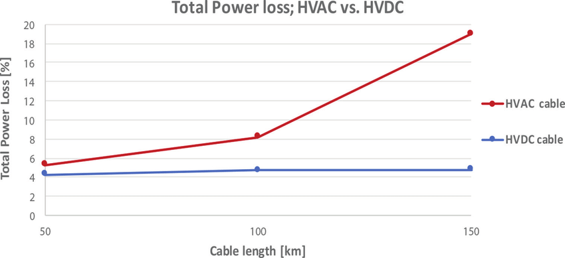
\includegraphics[width=0.7\textwidth]{pictures/hvdcVShvac.png}
		\label{fig:hvdc-hvac}
		\caption{Comparison of power losses in alternate and direct current cables. Courtesy of L. Våbenø \& O. T. Gudmestad, Int. J. of Energy Prod. \& Mgmt. \cite{design-install-hvdc}}
	\end{figure}
\end{comment}
\begin{figure}
	\centering
	\begin{tikzpicture}
		\node[anchor=south west,inner sep=0] (image) at (0,0,0) {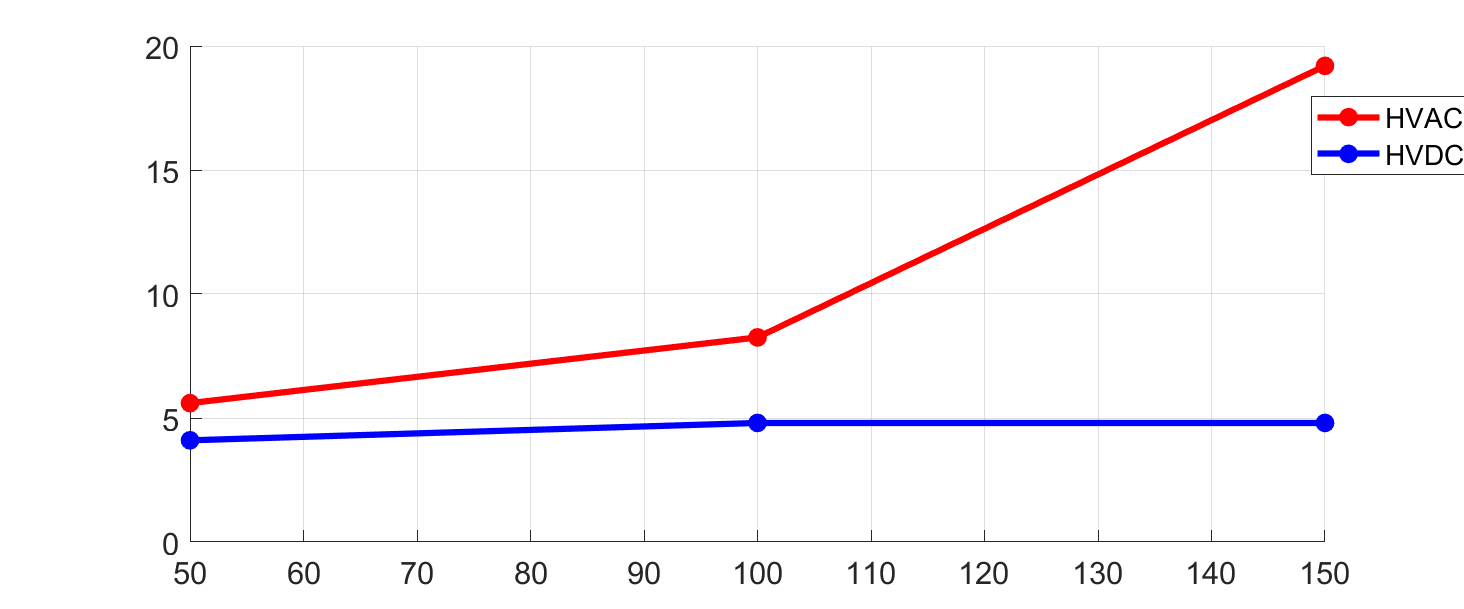
\includegraphics[width=0.7\textwidth]{pictures/hvdcVShvacp.png}};
		\begin{scope}[x={(image.south east)},y={(image.north west)}]
			\node (longdir) at (0.9,-0.02) {\footnotesize Cable length (Km)};
			\node (longdir) at (0.1,1.03) {\footnotesize Power losses (\%)};
		\end{scope}
	\end{tikzpicture}
	\caption{Comparison of (percentage) power losses in alternate and direct current cables. Data from \cite{design-install-hvdc}}
	\label{fig:hvdc-hvac}
\end{figure}
\begin{figure}
\begin{tikzpicture}
	\node[anchor=south west,inner sep=0] (image) at (0,0,0) {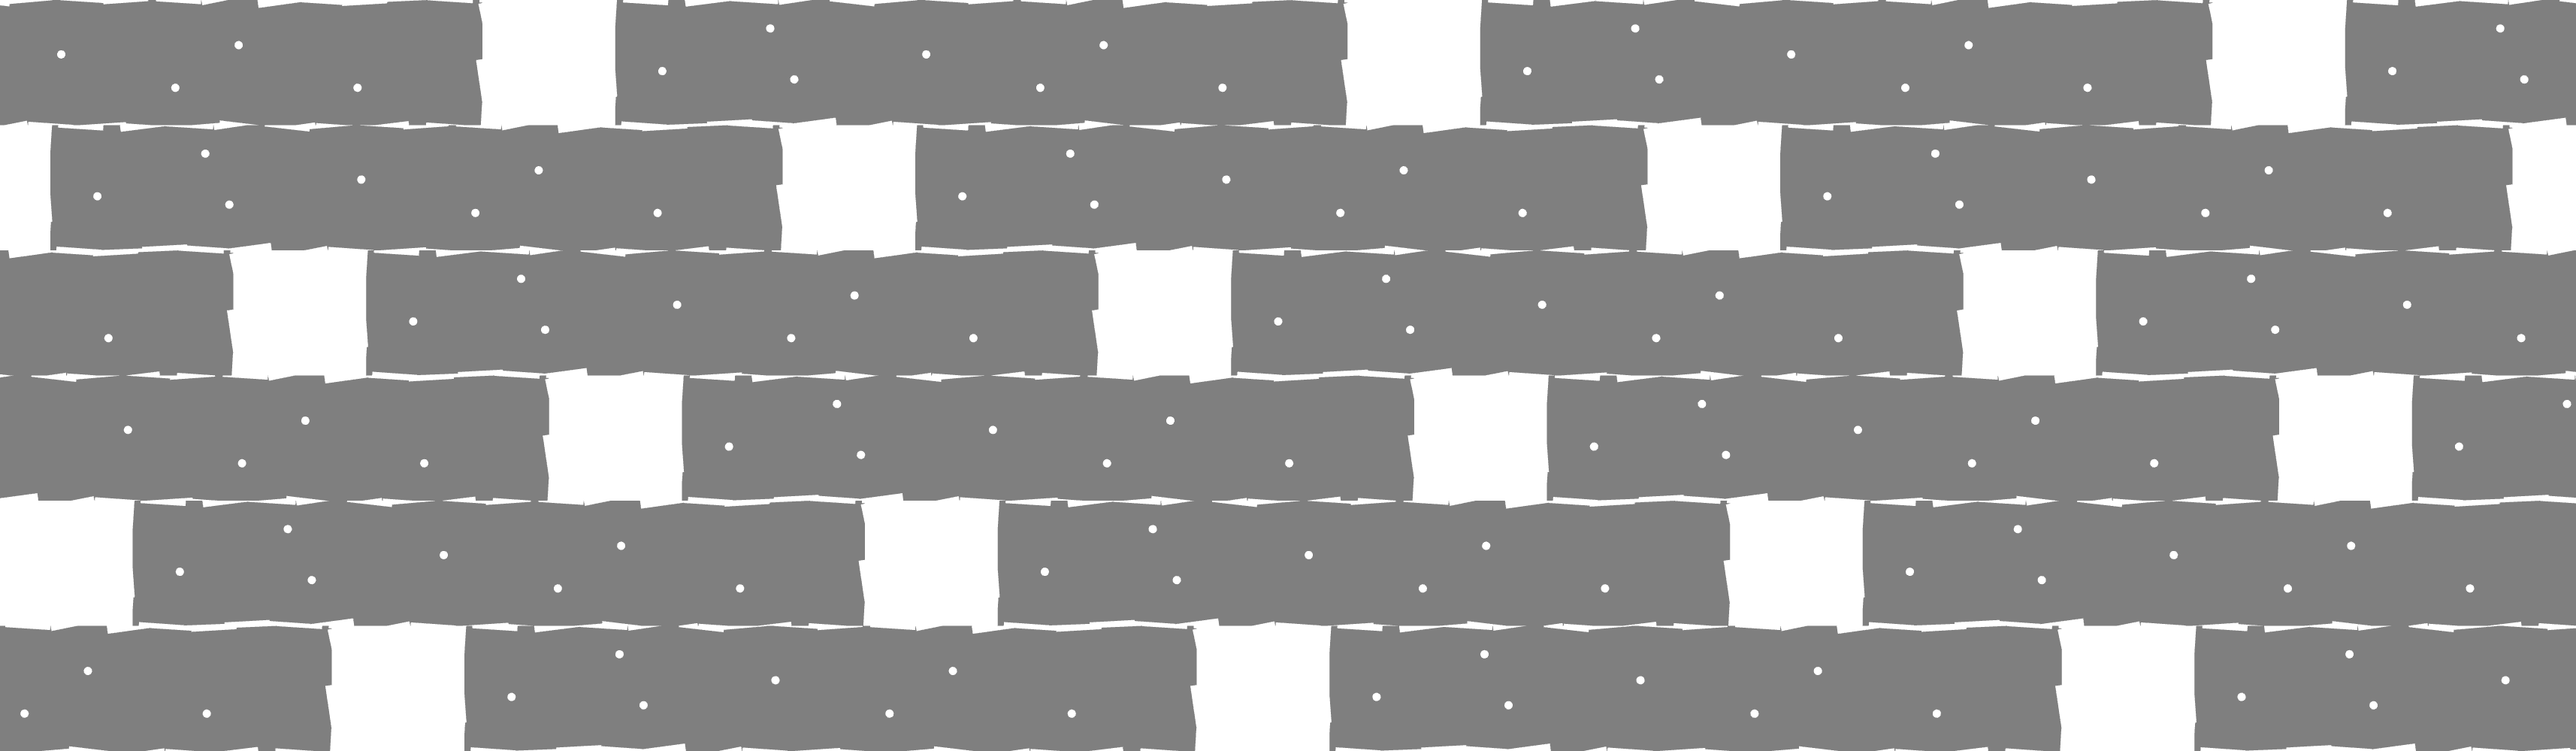
\includegraphics[width=0.7\textwidth]{pictures/MI_paper.png}};
	\begin{scope}[x={(image.south east)},y={(image.north west)}]
		\draw[thick,<->] (0.125,0) -- (0.18,-0);
		\draw[thick,<->] (0.5,0) -- (0.5,0.1666);
		\draw[thick,<->] (0.52,-0.05) -- (0.8,-0.05);
		\node (gapwidth) at (0.15,-0.1) {$10^{-3}$m};
		\node (gapheight) at (0.47,-0.06) {$10^{-4}$m};
		\node (tapelength) at (0.65,-0.12) {$10^{-2}$m};
		\node (tape) at (1.1,0.93) {Tape};
		\node (buttgap) at (1.1,0.75) {Butt gap};
		\node (channel) at (1.1,0.435) {Channel};
		\node (intersheetgap) at (1.15,0.16667) {Inter-sheet gaps};
		\draw[thick,->] (tape) -- (0.8,0.93);
		\draw[thick,->] (buttgap) -- (0.7,0.75);
		\draw[thick,->] (channel) -- (0.797,0.435);
		\draw[thick,->] (intersheetgap) -- (0.92,0.16667);
		\draw[thick,->] (0.4,-0.8) -- (0.9,-0.8);
		\draw[thick,->] (0.4,-0.8) -- (0.4,-0.5);
		\node (longdir) at (1.12,-0.8) {Cable longitudinal direction};
		\node (longdir) at (0.45,-0.4) {Cable radial direction};
	\end{scope}
\end{tikzpicture}
\caption{MI paper insulation structure, with approximate dimensions}
\end{figure}
\subsection{Polypropylene and Polyethilene Solid Insulation}
More recently, different technologies for the insulation system based on polyethilene and polypropylene have been proposed. These cables are easier to handle and lighter with respect to MI cables, representing a valid alternative, and are gaining popularity on the market. However from a modeling perspective they show a more complex behavior, as different non-linearities arise when the insulating dielectric is stressed with very high voltage, which make them more unpredictable. The reason of these non linearities is related to the charge trapping phenomena.
\subsection{Challenges for the future}
HVDC cables routinely undergo voltage changes in different ways when cables are switched on and off, or when power flow in the cable is inverted. This occurs in response to the varying energy requirements at different nodes within the network. Looking ahead, with the widespread use of renewable energy sources, which can be very intermittent according to weather conditions, we also expect current reversals in HVDC cables to become increasingly frequent. All of these transients critically test the resilience of the insulating material, and need to be studied \cite{hakonseththesis}.
\subsection{Mathematical models and numerical methods}
Mathematical models and numerical simulations can be an useful tool to estimate reliability of HVDC cables, in particular during the transient phase.\\
There are different dynamics to consider when modeling these materials, apart from those described by the usual Maxwell equations for a dielectric. First of all the slow polarization of the material, meaning that response of the dipoles to a variation of the electric field is not instantaneous. Then we have charge trapping phenomena, typical in polymer based materials. Finally, conductivity is in general not a constant, but a function of the electric field and the temperature \cite{time-dep-layered}.\\
Mathematical models can be classified by their complexity and ability to describe the dynamics previously mentioned. In section \ref{sec:mat-model} we report a fairly comprehensive model. Our main focus, however, will then be a simpler one, suitable for MI paper case, without charge trapping phenomena. In particular, it will be based on Maxwell equations and a Debye relaxation model for slow polarization. The Debye model consists in a superposition of polarization processes at different rates, ruled by ordinary differential equations. Its parameters need to be fitted according to experimental data.\\
It is interesting to note that, in research, this and other classes of electromagnetic problems have catalyzed the development of the so called \textit{Finite Difference Time Domain} with \textit{Auxiliary Differential Equation} method (ADE-FDTD) \cite{ADE-FDTD-thesis},\cite{ADE-FDTD-art}. The idea, starting from Maxwell equations, is to introduce auxiliary variables and associated differential equations reproducing the slow polarization effect. The solution proposed here is analogous to ADE-FDTD method, but also presents some differences. Here, for the spatial discretization, a finite element approach is adopted which will be presented later. Moreover, while in ADE-FDTD algorithms, the auxiliary variables are polarization vectors associated to a certain frequency (\(\mathbf{P}_k\)), here we use the simple polarization charges (\(\pi_k=\nabla \cdot\mathbf{P}_k\)).\\
On the other hand alternative approaches have been developed and successfully applied to dielectric materials, like the Occhini circuital model \cite{simulation-transient-HVDC}. This is strictly bound to the Debye model, and is very effective at simulating polarization 1-D problems. However applications are generally 3-D and non-homogeneous, motivating the finite element approach here presented.


\section{Mathematical Model}\label{sec:mat-model}
In this section we start introducing a simple model for dielectric materials coming directly from Maxwell equations with the assumption of electro-quasi-static regime. As anticipated, to obtain a more precise simulation, particularly in transient regimes, slow polarization must be taken into account. To this end Debye relaxation model is adopted. This will add to the original system a new pack of equations and variables describing the dynamics of polarization charges. In the next sections we will only focus on this model with slow polarization processes. Nonetheless  here we go further introducing a model for the conductivity, which is typically dependent on electric field intensity and on temperature. Finally we present a very general model considering also deep charge trapping phenomena, arising in polymer based insulating materials. We conclude presenting boundary conditions for the model with slow polarization processes.
\subsection{A first simple model}
We start from Gauss and Ampère-Maxwell laws

\begin{equation}
	\mathrm{div}\  \mathbf{D}  = \rho 
	\label{eq:Maxwell1}
\end{equation}
\begin{equation}
	\mathrm{curl}\ \mathbf{H} = \mathbf{j} + \dfrac{\partial \mathbf{D}}{\partial t}.
	\label{eq:Maxwell2}
\end{equation}
where \(\mathbf{j}\) is the drift current, associated to the moving free charges.\\
In the electro--quasi--static regime, introducing the electric potential \(\varphi\) it hods

\begin{equation} 
	\mathbf{E} = - \nabla \varphi.
	\label{eq:Epotential}
\end{equation}

Inside a dielectric material we have:
\begin{equation}
	\mathbf{D} = \varepsilon_{0} \mathbf{E} + \mathbf{P}
	\label{eq:D_composition}
\end{equation}
\begin{equation}
	\mathbf{j} = \sigma \mathbf{E}
	\label{eq:Ecurrent}
\end{equation}
where \(\sigma\) is the material conductivity.\\
For now we only consider instantaneous polarization of the material, so that 
\begin{equation}
	\mathbf{P} = \chi \mathbf{E}
\end{equation}
where \(\chi\) is the electric susceptibility. Now
\begin{equation}
	\mathbf{D} = \left( \varepsilon_0+\chi\right)\mathbf{E} = \varepsilon_0\varepsilon_r\mathbf{E}
	\label{eq:DandE}
\end{equation}
where \(\epsilon_r\) is the relative permittivity.\\
By substituting \eqref{eq:DandE} in \eqref{eq:Maxwell1}, using also \eqref{eq:Epotential}
\begin{equation}\label{eq:LEVEL0a}
	- \mathrm{div}\ \left( \varepsilon_{0} \varepsilon_{r}\ \nabla \varphi
	\right)  = \rho
\end{equation}
On the other hand if we apply the divergence operator to \eqref{eq:Maxwell2} the l.h.s vanishes, while on the r.h.s. we derive from \eqref{eq:Maxwell1}--\eqref{eq:Epotential}--\eqref{eq:Ecurrent}:
\begin{equation}\label{eq:LEVEL0b}
	\dfrac{\partial \rho}{\partial t} - \mathrm{div} \left(  \sigma \nabla \varphi\right) = 0
\end{equation}
Equations \eqref{eq:LEVEL0a}--\eqref{eq:LEVEL0b} together represent the simplest model for a dielectric material.
\subsection{Slow polarization}
The simple model just presented is valid as long as we only have instantaneous response of the material to the electric stimulus. Unfortunately this is rare, and non instantaneous response cannot be neglected in HVDC insulation systems. In other words the relation between \(\mathbf{P}\) and \(\mathbf{E}\) is not local in time and could be written as \begin{equation}
	\mathbf{P}(t) = \varepsilon_0 \int_{-\infty}^{t}\chi(t-\tau)\mathbf{E}(\tau)\mathrm{d}\tau
\end{equation}
This delayed response is usually treated with the so called Debye relaxation models. We consider \(\mathbf{P}\) to be the combination resulting from different polarization processes
\begin{equation}
	\mathbf{P} = \mathbf{P}_\infty +\sum_k \mathbf{P}_k
\end{equation}
where \(\mathbf{P}_\infty = \chi_\infty \mathbf{E}\) is the instantaneous polarization, and for each \(k\) it hods
\begin{equation} \label{eq:Polprocess}
	\tau_{k}\ \dfrac{\partial}{\partial t} \mathbf{P}_{k} =
	- \left( \varepsilon_{0} \chi_{k} \nabla \varphi + \mathbf{P}_{k}\right).
\end{equation}
Now we need same care to introduce these new equations to model \eqref{eq:LEVEL0a}--\eqref{eq:LEVEL0b}. Setting \(\pi_k = \mathrm{div}\mathbf{P}_k\) and 
\begin{equation}
	\mathbf{D} = \varepsilon_0 \mathbf{E} + \mathbf{P} = \varepsilon_0\varepsilon_\infty \mathbf{E} + \sum_k \mathbf{P}_k
\end{equation}
with similar substitutions as in the previous case we obtain the following model which has been implemented in this work.\\
\begin{subequations}\label{eq:finalmodel}
	\begin{alignat}{2}[left=\empheqlbrace]
		\dfrac{\partial \rho}{\partial t} & - \mathrm{div} \left( \sigma \nabla \varphi\right) &&= 0\\[3mm]
		%%
		&- \mathrm{div}\ \left( \varepsilon_{0} \varepsilon_{\infty}\ \nabla \varphi
		\right) - \rho +  \sum_{k} \pi_{k} &&= 0\\[3mm]
		%%
		\tau_k	\dfrac{\partial \pi_{k} }{\partial t} &+ \mathrm{div}\ \left(\varepsilon_{0} \chi_{k}\ \nabla \varphi
		\right) + \pi_{k} &&= 0
	\end{alignat}
\end{subequations}
Note that we renamed \(\varepsilon_r\) to \(\varepsilon_\infty\), since relative permittivity now depends on the frequency. 
\subsection{Conductivity}
In general, conductivity depends on electric field intensity and temperature. An appropriate model follows:
\begin{equation}\label{eq:conductivitymodel}
	\sigma = (1-a)\ \sigma_{1} \left(|\nabla \varphi|, T \right) +
	a\ \sigma_{0} \left( T \right)
\end{equation}
with 
\begin{equation}\label{eq:conductivitymodelaux}
	\tau_{a} \dfrac{\partial a}{\partial t} = \bar{a}\left(|\nabla \varphi|\right) - a.
\end{equation}

\[
\bar{a} = \begin{cases}
	0, \; |\nabla \varphi| > e_{tr}\\[3mm]
	1, \; |\nabla \varphi| \le e_{tr}
\end{cases}
\]

\[
\dfrac{1}{\tau_{a}} = \begin{cases}
	\dfrac{\kappa+1}{c}\ \sqrt[\kappa+1]{a(t)}, \; |\nabla \varphi| > e_{tr}\\[3mm]
	\dfrac{1}{\bar{\tau}_{a}}, \; |\nabla \varphi| \le e_{tr}
\end{cases}
\]
where \(\bar{a}\), \(e_{tr}\), \(\kappa\), \(c\) and \(\bar{\tau}_a\) are physical constants of the material. Therefore, modeling \(\sigma\) leads to an additional differential equation to \eqref{eq:finalmodel}.
\subsection{Trapping and de-trapping}
Model \eqref{eq:finalmodel} gives good results when applied to MI paper insulation systems. However it fails with polymeric materials, as new dynamics arise.\\
Here a characteristic phenomenon are the charge deep traps, which are thought to have chemical origin. This leads to an ad-hoc treatment of the free charge density:
\begin{equation}\label{eq:freechargetraps}
	\rho = q\,(p-n-b)
\end{equation}
where \(q\) is the positive elementary charge, \(n\) are the negative mobile charges per unit volume, \(p\) are the positively charged trap states per unit volume and \(b\) are the negative trapped charges, always per unit volume. \(p\) is assumed fixed in time
\begin{equation}
	\dfrac{\partial p}{\partial t} = 0
\end{equation}
Trapping and de-trapping of \(b\) needs instead to be modeled. Depth of traps can be associated to the amount of energy required to extract a retained particle \cite{circuitalmodel}. Experiments suggest that the distribution of the density of states (DOS)  for deep traps is a superposition of Gaussian distributions. However to limit the complexity, a single Gaussian distribution is assumed here:
\begin{equation}
	g(x) = \dfrac{N}{\alpha \sqrt{2 \pi}} \exp \left( -\dfrac{\left(x+\Delta \mathcal{E}\right)^{2}}
	{2 \alpha^{2}} \right)
\end{equation}
where \(N\) represents the total number of charges that deep traps can retain per unit volume. \(\Delta \mathcal{E}\) represents the mean trap depth, and \(\alpha^2\) its variance.\\
It is reasonable to assume that charges fill the deeper traps first. Thus we can express the amount of trapped charges \(b\) as a function of the max level of energy \(\mathcal{E}_{max}\):
\begin{equation}
	\dfrac{b}{N} = \displaystyle \int_{-\infty}^{\mathcal{E}_{\mathrm{max}}} \dfrac{g(x)}{N}\, \mathrm{d}x =
	\mathop{\int_{-\infty}^{\mathcal{E}_{\mathrm{max}}}} \frac{1}{\alpha \sqrt{2 \pi}} \exp \left( -\dfrac{\left(x+\Delta \mathcal{E}\right)^{2}}
	{2 \alpha^{2}} \right)\mathrm{d}x
	=: F\left(\mathcal{E}_{\mathrm{max}}\right)
\end{equation}
Knowing \(\Delta \mathcal{E}\) and \(\alpha\), we can define \(\mathcal{E}_\mathrm{av}\) the average occupied level of energy and relate it to \(\mathcal{E}_{\mathrm{max}}\):
\begin{equation}
	\mathcal{E}_{\mathrm{av}} := \dfrac{\displaystyle \int_{-\infty}^{\mathcal{E}_{\mathrm{max}}} x\ g(x)\, \mathrm{d}x} {\displaystyle \int_{-\infty}^{\mathcal{E}_{\mathrm{max}}} g(x)\, \mathrm{d}x} =:
	\Gamma\left(\mathcal{E}_{\mathrm{max}}\right)
\end{equation}
Then, trivially:
\begin{equation}
	\mathcal{E}_{\mathrm{av}} = \Gamma\left(F^{-1}\left(\dfrac{b}{N}\right)\right)
\end{equation}
Charge trapping rate depends on how many trap states are unoccupied, on the drift current, and on the traps cross-section \(c_s\)[\(\mathrm{m}^2\)]:
\begin{equation}\label{eq:trap}
	\dot{b}_c = c_s|\mathbf{j}|(N-b)
\end{equation}
While charge trapping begins as soon as the voltage is turned on, de-trapping is typically a slower process: the rate at which charges escape from traps depends on the occupied energy level. In the proposed model:
\begin{equation}\label{eq:detrap}
	\dot{b}_e = w_0\ b\ \exp \left(\dfrac{\mathcal{E}_{\mathrm{av}} \left( \dfrac{b}{N}\right) + \Delta \mathcal{E}}{\kappa_\mathrm{B} T }\right) =: w\left(\dfrac{b}{N}\right)b
\end{equation}
where \(w_0\) is the attempt-to-escape rate when states are full, \(T\) is the temperature and \(\kappa_\mathrm{B}\) is the Boltzmann constant.\\
Combining \eqref{eq:trap}--\eqref{eq:detrap}:
\begin{equation}
	\dot{b} = \dot{b}_c -\dot{b}_e = c_s|\mathbf{j}|(N-b) - w_0\ b\ \exp \left(\dfrac{\mathcal{E}_{\mathrm{av}} \left( \dfrac{b}{N}\right) + 
		\Delta \mathcal{E}}{\kappa_\mathrm{B} T }\right)
\end{equation}
Finally, combining all the elements introduced so far, the following model is derived:

\begin{subequations}\label{eq:fullmodel1}
	\begin{align}[left=\empheqlbrace]
		&- \mathrm{div}\ \left( \varepsilon_{0} \varepsilon_{\infty}\ \nabla \varphi
		\right)  = q \left( p - n - b \right) -  \sum_{k} \pi_{k} \\[2.5mm]
		%%
		&\dfrac{\partial n}{\partial t} + \mathrm{div} \left(  \dfrac{\sigma}{q} \nabla \varphi\right) =
		- c_s|\mathbf{j}| \left(N - b\right) +
		w \left( \dfrac{b}{N}\right) \ b\\[2.5mm]
		%%
		&\dfrac{\partial b}{\partial t} = c_s |\mathbf{j}| \left(N - b\right) - 
		w \left( \dfrac{b}{N}\right) \ b \\[2.5mm]
		%%
		&\tau_{i}\ \dfrac{\partial}{\partial t} \pi_{i} =
		\dfrac{\chi_{i}}{\varepsilon_{0}} \left( q \left( p - n - b \right) -  
		\sum_{k} \pi_{k} \right) - \pi_{i}\\[2.5mm]
		%%
		&\tau_{a} \dfrac{\partial a}{\partial t} = \bar{a}\left(|\nabla \varphi|\right) - a
	\end{align}
\end{subequations}
\begin{equation}\label{eq:fullmodel2}
	\begin{cases}
		\sigma = (1-a)\ \sigma_{1} \left(|\nabla \varphi|, T \right) +
		a\ \sigma_{0} \left( T \right)\\[3mm]
		\bar{a} = \begin{cases}
			0, \; |\nabla \varphi| > e_{tr}\\[3mm]
			1, \; |\nabla \varphi| \le e_{tr}
		\end{cases}
	\end{cases}
\end{equation}
Note that starting from \eqref{eq:fullmodel1}--\eqref{eq:fullmodel2} and taking the following assumptions:
\begin{equation}
\begin{cases}
	a = 0\\
	N\rightarrow 0
\end{cases}
\end{equation}
we retrieve \eqref{eq:finalmodel}
\subsection{Boundary conditions}
We briefly discuss typical boundary conditions for \eqref{eq:finalmodel}.\\
The only variable appearing under space differential operator is the electric potential \(\varphi\). Therefore it as also the only variable to which b.c. are meaningful. Typically the dielectric is interposed between different contacts at different voltages. It comes natural to impose Dirichlet b.c. on the contacts. On the other sides of the domain natural b.c. are adopted:
\begin{equation}\label{eq:LEVEL1Bc}
	\left\{\begin{aligned}
		\left.\varphi\right. = \varphi_D\ &\ \mathrm{on}\ \Gamma_D\\[3mm]
		-\left.\left(\sigma \nabla  \varphi \cdot n\right) = 0\right. &\ \mathrm{on}\ \Gamma_N
	\end{aligned}\right.
\end{equation}
Normally \(\Gamma_D\) is the union of contact surfaces \(\Gamma_k\).

\section{Numerical Discretization}
We subdivide this section in time semi-discretization and space discretization.

\subsection{Time semi-discretization}\label{sec:time-discr}
Consider the system of equations \eqref{eq:finalmodel}: it consists in a set of \(m+2\) PDEs in the \(m+2\) variables \(\varphi\), \(\rho\), \(\pi_i\) for \(i=1,...,m\). The Implicit Euler method can be applied to discretize the problem in time. Given time step magnitude \(\Delta t\) and the the solution at time step \(n\) \((\varphi^n,\rho^n,\pi_i^n)\) we solve the following system:
\begin{subequations}
	\begin{alignat}{2}[left=\empheqlbrace]
		&\rho^{n+1}-\nabla\cdot\left(\Delta t \nabla \varphi^{n+1} \right) &&= \rho^n\\[3mm]
		%%
		&-\nabla\cdot \left(\epsilon_0\epsilon_\infty\nabla\varphi^{n+1}\right) -\rho^{n+1}+\sum_i\pi_i^{n+1} &&=0\\[0mm]
		%%
		&\left(1+\frac{\Delta t}{\tau_i}\right)\pi_i^{n+1} + \nabla\cdot\left(\Delta t\epsilon_0\chi_i\nabla\varphi^{n+1}\right) &&= \pi_i^n\\[3mm]
		%%
		&\varphi^{n+1}=V_k(t^{n+1})\ \mathrm{on}\ \Gamma_{c_k} \forall\ k\\
		%%
		&\nabla\varphi^{n+1}\cdot \mathbf{n}=0\ \mathrm{on}\ \partial \Omega \setminus \Gamma_c
	\end{alignat}
\end{subequations}
where $V_k$ and $\Gamma_{c_k}$ are respectively the voltage imposed on contact $k$ and its surface, and $\Gamma_c=\cup_k \Gamma_{c_k}$.\\
We also adopt an adaptive time step method: \(\Delta t\) is not fixed once for all, but may be adjusted according to an error estimate: given the last solved time step magnitude \(\Delta t^k\), the estimated error \(err\) and tolerance \(tol\), we set \(\Delta t^{k+1}=\Delta t^k\,\left(\frac{err}{tol}\right)^{-1/2}0.9\) if \(err < tol\), otherwise we halve \(\Delta t^k\) and we repeat the last iteration until \(err < tol\).\\
To ease post-processing however, we want to save the solution in regular steps. This necessity leads to an external loop iterating through fixed time steps \(\Delta t\) with a nested loop marching from \(t\) to \(t+\Delta t\) using the adaptive time step method. For the complete algorithm see section \ref{sec:timecycle}.
\paragraph{Error estimate} Consider a generic first order advancing scheme for the variable \(x\) defined by \(f(x^{n+1},x^n, \Delta t)=0\) and define the time-advance operator \(g\) such that \(x^{n+1}=g(x^n,\Delta t)\). An error estimate can be done comparing the two solutions \(x_1=g(x^n,\Delta t)\) and \(x_2=g(g(x^n,\Delta t/2),\Delta t/2)\). In our case, given the solutions 1 and 2, we compute the correspondent total conduction currents through one contact \(I_{cond\, 1}\) and \(I_{cond\,2}\) and compare the relative error \((I_{cond\,1}+I_{cond\,2})/I_{cond\,2}\) with a predefined tolerance.

\subsection{Spatial discretization}
Being the applications of interest 3-dimensional, in the code we considered a cubic domain. Discretization is managed by bim++ library, which is able to handle non conforming cartesian meshes, with regular hexahedral cells, through an octree data structure. Here is no place to introduce this library so we go straight to the discreization starting from a uniform grid and then refining it locally in non conforming way. For further information please refer to \cite{thesis-pasquale-africa}. 
\paragraph{Uniform grid case}
We consider the partition \(\tau_h\) of the domain \(\Omega\) in \(N\) elements:
\begin{equation}
	\tau_k=\left\{\mathcal{K}^k\right\}_{k=1}^N,\ \ \Omega_h=\bigcup_{k=1}^N \mathcal{K}^k \subseteq \Omega
\end{equation}
Then we define the space of trilinear polynomials:
\begin{equation}
	\mathbb{Q}_{m,n,l}(\Omega)=\left\{q:\Omega\rightarrow\mathbb{R}, q(x,y,z)=\sum_{i\leq m,j\leq n,k\leq l}a_{ijk}x^iy^jz^k\ \forall (x,y,z)\in\Omega \right\}
\end{equation}
Now the space for the discretization of our problem can be written:
\begin{equation}
	Q_h^1(\tau_h) = \left\{u\in C^0\left(\overline{\Omega}_h\right),\ u|_{\mathcal{K}^k}\in\mathbb{Q}_{1,1,1}\left(\mathcal{K}^k\right)\ \forall \mathcal{K}^k\in \tau_h \right\}
\end{equation}
At this point a lagrangian basis for the space can be obtained in the same way as for continuous Galerkin finite element method.
\paragraph{Non uniform mesh}
\begin{figure}\captionsetup[subfloat]{labelformat=empty}
	\subfloat[]{
		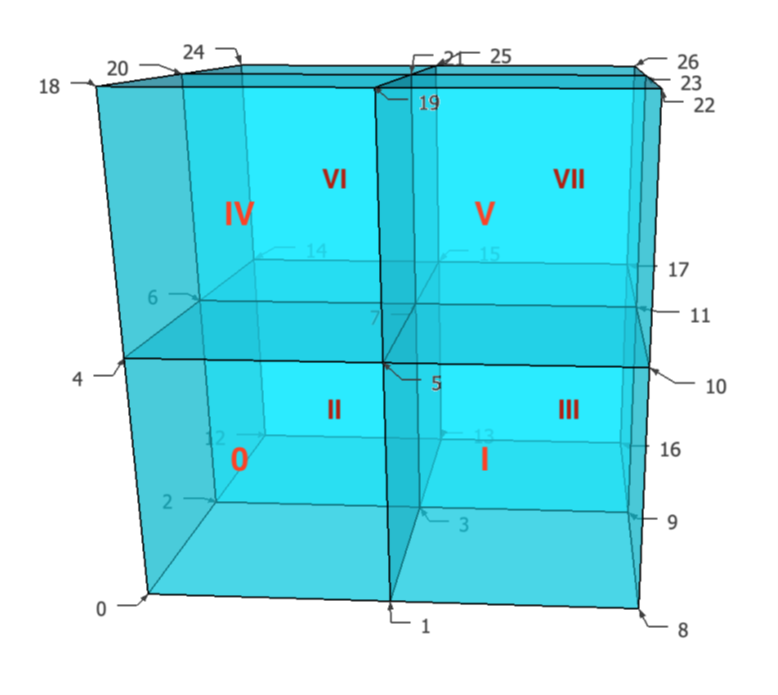
\includegraphics[width=0.49\textwidth]{pictures/octant_not_refined.png}
	}
	\subfloat[]{
		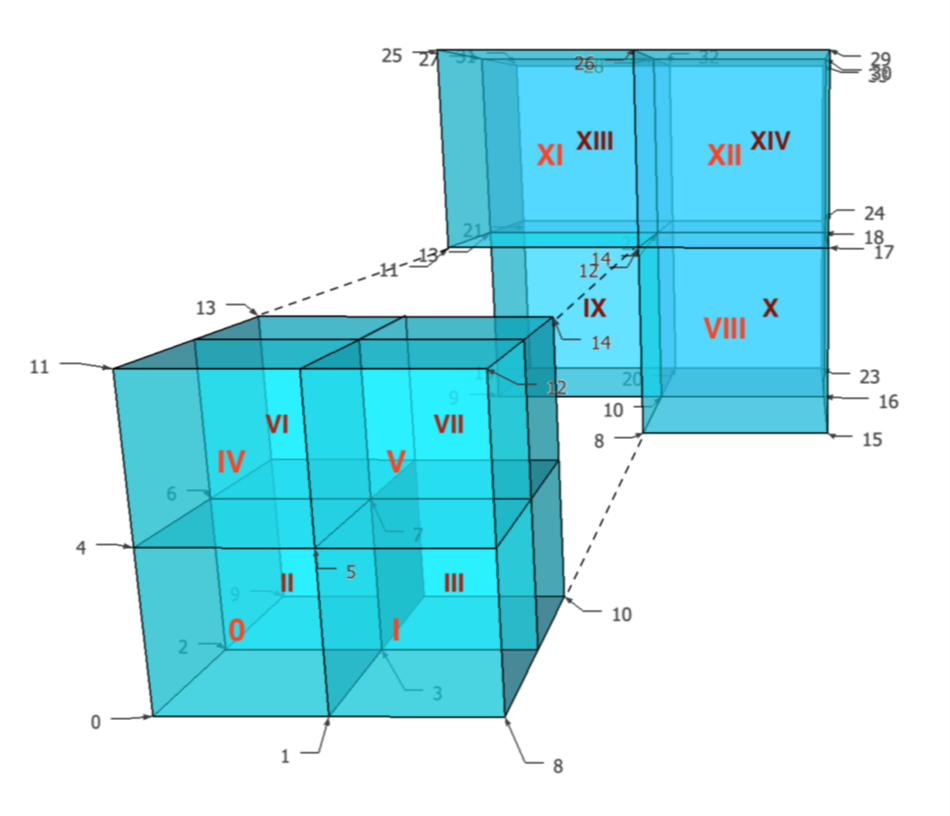
\includegraphics[width=0.49\textwidth]{pictures/octant_refined.png}
	}
	\caption{Refinement procedure of a cell. On the left the uniform grid, on the right the grid refined in the cell 0.}
	\label{fig:octant_refinement}
\end{figure}\captionsetup[subfloat]{labelformat=parens}
To refine the grid in a specific (regular cube-shaped) cell, we cut it into eight similar cube-shaped cells as shown in figure \ref{fig:octant_refinement} where the refinement procedure of cell 0 is displayed. At the end of the process new vertices appear, but not all of them correspond to new degrees of freedom: vertices that are internal to the domain and are not the vertices of all adjacent cells are called hanging nodes and do not introduce degrees of freedom. For simplicity consider the refinement of a singular cell \(\mathcal{K}\) internal to the mesh (no edge on borders). We describe now the procedure to obtain the new function space by building the new set of basis functions. Let \(\tau_h\) be the original uniform domain discretization and \(\overline{\tau}_h\) the discretization obtained by uniformly refining \(\tau_h\). By refining the cell \(\mathcal{K}\) we obtain only one new degree of freedom in its centre. We associate it to the same base function it would have in the uniform refinement of the whole mesh \(\overline{\tau}_h\), say \(\overline{\varphi}_8\in Q_h^1(\overline{\tau_h})\). At the same time we replace the basis functions \(\varphi_i \in Q_h^1(\tau_h,\ i=0,...,7\), associated to the vertices of \(\mathcal{K}\), with \(\tilde{\varphi}_i=\varphi_i-\frac{1}{8}\overline{\varphi}_8\). The new set of basis functions \(\tilde{\varphi}_i\) where \(\tilde{\varphi}_i\) is defined as above for \(i=1,...,7\), \(\tilde{\varphi}_8=\overline{\varphi}_8\) and \(\tilde{\varphi}_i = \varphi_i\ \forall i \notin 1,...,8\) (outside \(\mathcal{K}\) they are left unchanged) identifies a new linear space \(\tilde{Q}_h^1(\tilde{\tau}_h)\). Moreover \(\sum_{i=1}^N\tilde{\varphi}_i=1\) and \(\Tilde{\varphi}_i(x_j)=\delta_{ij}\ \forall x_j\in \tilde{X}\), \(\tilde{X}\) being the set of nodes of \(\tilde{\tau_h}\).
\subsection{Discrete weak formulation}
Now that we gave defined an appropriate functional space we can introduce a weak formulation for problem \eqref{eq:finalmodel}. Defining \(Q_h\) the functional space just presented applied to our domain \(\Omega_h\), setting \(p\) the number of polarization processes, we state:\\
Given \((\rho^n,\ \varphi^n,\ \pi^n_1,\ ...,\ \pi^n_p)\in Q^{2+p}_h\) the solution at time \(t^n\), find \((\rho^{n+1},\ \varphi^{n+1},\ \pi^{n+1}_1,\ ...,\ \pi^{n+1}_p)\in Q^{2+p}_h\) such that:
\begin{subequations}\label{eq:Gal-form}
	\begin{alignat}{2}[left=\empheqlbrace]
		&\int_{\Omega_h}\rho^{n+1}v_1\ \mathrm{d}\Omega_h + \int_{\Omega_h}\left(\Delta t \sigma \nabla \varphi^{n+1} \right)\cdot\nabla v_1\ \mathrm{d}\Omega_h &&= \int_{\Omega_h}\rho^n v_1\ \mathrm{d}\Omega_h\\[3mm]
		%%
		&\int_{\Omega_h}\left(\epsilon_0\epsilon_\infty\nabla\varphi^{n+1}\right) \cdot \nabla v_2\ \mathrm{d}\Omega_h - \int_{\Omega_h}\rho^{n+1}v_2+\sum_i\int_{\Omega_h}\pi_i^{n+1}v_2\ \mathrm{d}\Omega_h &&=0\\[0mm]
		%%
		&\int_{\Omega_h}\left(1+\frac{\Delta t}{\tau_i}\right)\pi_i^{n+1}v_i\ \mathrm{d}\Omega_h - \int_{\Omega_h}\left(\Delta t\epsilon_0\chi_i\nabla\varphi^{n+1}\right) \cdot \nabla v_i\ \mathrm{d}\Omega_h &&= \int_{\Omega_h}\pi_i^n v_i\ \mathrm{d}\Omega_h\\[3mm]
		%%
		&\varphi^{n+1}=V_k(t^{n+1})\ \mathrm{on}\ \Gamma_{c_k} \forall\ k
	\end{alignat}
\end{subequations}
for all test functions \((v_1,...,v_{p+2}) \in Q_h^{2+p}\). Note that no boundary term appears apart from Dirichlet conditions for \(\varphi^{n+1}\). Charges accumulating on the domain border will be approximated by charge volumetric densities next to it, while Dirichlet b.c. for \(\varphi\) are enforced directly in the matrix and in the r.h.s..
\section{Code}
The code developed in this work is available at \url{https://github.com/lucaedomosconi/HVDC}. It implements model \eqref{eq:finalmodel} and is based, among the others, on the following third party libraries:
\begin{itemize}
	\item \textbf{bim++}: available at \url{https://github.com/carlodefalco/bimpp}, provides the utilities to generate and handle octree structured non-conforming cartesian meshes. All of its data structures and functions are optimized for parallel computing with MPI.
	\item \textbf{mumps}: provides a direct linear solver for sparse matrices, optimized for parallel running with MPI (see \url{https://mumps-solver.org/index.php}).
	\item \textbf{octave}: needed to export solutions to be post-processed with \textbf{Paraview}.
\end{itemize}
The application outputs the spatial distribution of variables every fixed time step in gz files that need to be post-processed in octave and visualized in Paraview. Moreover it provides some useful features handled through the parameter file:
\begin{itemize}
	\item Plugin architecture to define
	\begin{itemize}
		\item Templates of tests with different geometries and grids.
		\item The transient to apply.
	\end{itemize}
	\item Output of info about currents and charges in the material;
	\item Output of info about time-stepping algorithm, like error and computational time.
	\item Saving of temporary solutions to allow stopping a resuming a simulation later.
\end{itemize}

\subsection{Code structure}
The main code is located in \texttt{HVDC\_main.cpp}. Plugin source files are found in a dedicated folder. Here we report the code structure and the file dependency tree.
\begin{figure}[h]
\begin{minipage}{5cm}
	\caption*{Code Structure}
\end{minipage}\\
\begin{minipage}[t]{7cm}
	\small
	\begin{verbatim}
		HVDC/
		|-include/
		|  |-GetPot
		|  |-simple_connectivity_3d.h
		|  |-json_fun.h
		|  |-currents_comp.h
		|-json/include/nlohmann/json.hpp
		|-script/m/
		|  |-export_phi_rho_p1_3.m
		|-src/
		|  |-plugins/
		|  |  |-generic_factory.cpp
		|  |  |-generic_factory.h
		|  |  |-generic_test.h
		|  |  |-generic_voltage.h
		|  |  |-tests.h
		|  |  |-tests.cpp
		|  |  |-MI_paper.h
		|  |  |-MI_paper.cpp
		|  |  |-voltages.h
		|  |  |-voltages.cpp
		|  |-HVDC_main.cpp
		|  |-MakeFile
	\end{verbatim}
\end{minipage}
\end{figure}
\begin{figure}[h]
\begin{minipage}{\textwidth}
	\caption*{File dependency tree}
\end{minipage}\\
\begin{minipage}{\textwidth}
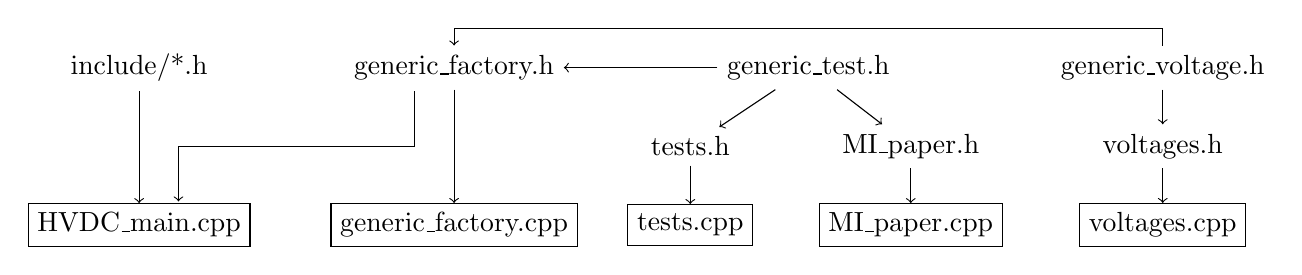
\begin{tikzpicture}
	\node (s1) at (0,2) {include/*.h};
	\node[draw,rectangle] (s2) at (0,0) {HVDC\_main.cpp};
	\node (s3) at (4,2) {generic\_factory.h};
	\node[draw,rectangle] (s4) at (4,0) {generic\_factory.cpp};
	\node (s5) at (8.5,2) {generic\_test.h};
	\node (s6) at (7,1) {tests.h};
	\node[draw,rectangle] (s7) at (7,0) {tests.cpp};
	\node (s8) at (13,2) {generic\_voltage.h};
	\node (s9) at (13,1) {voltages.h};
	\node[draw,rectangle] (s10) at (13,0) {voltages.cpp};
	\node (s11) at (9.8,1) {MI\_paper.h};
	\node[draw,rectangle] (s12) at (9.8,0) {MI\_paper.cpp};
	\path
	(s1) edge[->] (s2)
	(s3) edge[->] (s4)
	(s5) edge[->] (s6)
	(s6) edge[->] (s7)
	(s8) edge[->] (s9)
	(s9) edge[->] (s10)
	(s5) edge[->] (s11)
	(s11) edge[->] (s12)
	(3.5,1.7) edge[-] (3.5,1)
	(3.5,1) edge[-] (0.5,1)
	(0.5,1) edge[->] (0.5,0.3)
	(s5) edge[->] (s3)
	(s8) edge[-] (13,2.5)
	(13,2.5) edge[-] (4,2.5)
	(4,2.5) edge[->] (s3)
	;
\end{tikzpicture}
\end{minipage}
\end{figure}

\subsection{Parameter file}
Parameters of a simulation are set in the parameter file. A parameter file may contain different tests to execute in sequence. Each test is a json object subdivided into three sections: physics, algorithm and output.\\
\begin{minipage}{\textwidth}
	\vspace{3mm}
	\small
	\begin{verbatim}
		physics
		    epsilon_0 -> dielectric constant in vacuum
		    physics_plugin -> name of the plugin containing the test
		    plugin_test_index -> identifies the test to use in the plugin
		    plugin_params : {} -> object containing physical constants used by the test functions
	\end{verbatim}
	\vspace*{0mm}
\end{minipage}\\
Note that we have to specify a plugin, a test template inside it and a compatible list of parameters.\\
\begin{minipage}{\textwidth}
	\vspace{3mm}
	\small
	\begin{verbatim}
		algorithm
		    possibly some parameters for the mesh generation like  {
		        num_refinements -> used to generate a uniform mesh
			    maxlevel -> max local level of refinement for a mesh
		    }
		    T -> Full time: the application will simulate the evolution of the problem from time = 0
		         to time = T
		    biggest_time_step -> fixed time step magnitude; how often the application outputs the
		                         solution
		    initial_dt_for_adaptive_time_step -> magnitude of first time step in the Adative Time
		                                         Step Algorithm
		    tol_of_adaptive_time_step -> tol of relative error of conduction current
		    voltage_plugin -> name of the plugin containing the voltage function
		    voltage_name -> name of the function V(t)
		    voltage_plugins_params : {} -> contains parameters of the voltage function
		    start_from_solution -> if true the application will resume a previous simulation from a
		                           temporary solution
		    save_temp_solution -> if true the application will save the current solution and allow
		    the user to resume the simulation later
		    temp_sol : {} -> contains: {
		        file_of_starting_solution -> (if start_from_solution = true) file name of the
		                                     solution to resume the simulations
		        save_every_n_steps -> tells how frequently should the application save the
		                              temporary solution
		    }
	\end{verbatim}
\end{minipage}\\
\begin{minipage}{\textwidth}
	\vspace{3mm}
	\small
	\begin{verbatim}
		output
		    save_sol -> if true, the application saves the solution to be exported with octave
		    compute_charges_on_border -> if true, the application outputs in a file the different
		    charges on the contact (1)
		    save_cond_currents -> if true, enables the computation of conduction currents
		    save_error_and_comp_time -> if true, tracks error of the adaptive time step and
		                                computational times
	\end{verbatim}
\end{minipage}\\

\subsection{Time stepping}\label{sec:timecycle}
As exposed in section \ref{sec:time-discr} we aim at saving a solution every fixed time step \(\Delta t\). At the same time we use ad adaptive time-stepping approach inside the regular time step, that is, to advance from \(t^n\) to \(t^n+\Delta t\). This introduced some technicalities to care of, namely how to choose the time step magnitude to start a new "macro" time step. Choosing a very small value is obviously an expensive option. In this implementation, experience from the last resolved macro time step is used to prompt a starting \(dt\) for the next one. In Algorithm \ref{alg:adaptive-time-step} the complete time cycle run in the execution of the program is reported.

\begin{algorithm}
	\caption{Time cycle}
	\label{alg:adaptive-time-step}
	\begin{algorithmic}[1]
		\STATE T $\leftarrow$ full time;
		 $\Delta t\ \leftarrow$ fixed time step;
		 $dt\ \leftarrow$ small initial time step;
		 tol $\leftarrow$ tolerance;
		\STATE $t_{is}\ \leftarrow\ 0$;
		 $dt_{start}\ \leftarrow\ dt$;
		 truncate $\leftarrow$ false;
		 exit\_loop $\leftarrow$ false;
		 sol $\leftarrow$ last compute solution;
		\STATE \COMMENT{global regular time stepping}
		\WHILE{Time $<$ T}
			\STATE{exit\_loop  $\leftarrow$ false;}
			\STATE{truncate $\leftarrow$ false;}
			\STATE{$dt\ \leftarrow\ dt_{start}$;}
			\STATE{$t_{is}\ \leftarrow\ 0$;}
			\STATE \COMMENT{adaptive time-stepping}
			\WHILE{exit\_loop = false}
				\STATE{sol1 $\leftarrow$ time\_advance(sol, $dt$)};
				\STATE{sol2 $\leftarrow$ time\_advance(time\_advance(sol, $dt/2$), $dt/2$);}
				\STATE{error $\leftarrow$ compute\_error(sol1,sol2);}
				\IF{error < tol \OR $dt<dt_{min}$}
					\STATE{$t_{is}\ \leftarrow\ t_{is}+dt$;}
					\STATE{sol $\leftarrow$ sol2;}
					\IF{$t_{is}>\Delta t$}
						\STATE{Time = Time $+dt$;}
						\PRINT sol;
						\STATE{exit\_loop $\leftarrow$ true;}
					\ENDIF
					\STATE{$dt\ \leftarrow$ max($dt_{min}$, $0.9\,(\mathrm{error/tol})^{-1/2}$)}
					\IF{truncate = false}
						\STATE{$dt_{start}\ \leftarrow\ 0$}
					\ENDIF
					\STATE{$dt_{start}\ \leftarrow$ min($\Delta t$, max($dt_{start}$, $dt$))}
					\IF{$dt > \Delta t - t_{is}$}
						\STATE{$dt=\Delta t - t_{is}$}
						\STATE{truncate = true}
					\ENDIF
				\ELSE
					\STATE{$dt\ \leftarrow\ dt/2$}
					\STATE{$dt_{start}\ \leftarrow\ 0$}
				\ENDIF
			\ENDWHILE
		\ENDWHILE
	\end{algorithmic}
\end{algorithm} 

\subsection{Plugins}
As already mentioned plugins were used to contain the test specific functions and the evolution in time of voltage applied at one of the contacts. The source files are located in the \texttt{plugins} directory. 
\begin{itemize}
	\item \texttt{generic\_test.h} and \texttt{generic\_voltage.h} define the classes \texttt{generic\_test} and \texttt{generic\_voltage} respectively, with a set of virtual functions. The two files are included both in \texttt{HVDC\_main.cpp} and in plugins headers \texttt{tests.h} and \texttt{voltages.h}. They basically work as interface for the main program to call actual test functions defined elsewhere.
	\item \texttt{tests.h} and \texttt{voltages.h} contain a set of test and voltage classes inheriting from \texttt{generic\_test} and \texttt{generic\_voltage}. Object of these classes can be built by a factory and used in the main.
	\item \texttt{generic\_factory.h} and \texttt{generic\_factory.cpp} implement an abstract factory with the single-tone technique.
	\item Finally, to let the plugin mechanism work, when the dynamic libraries are loaded, \texttt{tests.cpp} and \texttt{voltages.cpp} guarantee auto-loading of the chosen test and voltage constructors in the factory. 
\end{itemize}
\section{Currents computation}
Just as with any dielectric material, we can distinguish between conduction current and displacement current:
\begin{itemize}
	\item \textit{Conduction current} or drift current, is generated by free charges moved by the electric field. It can be determined through the gradient of the electric potential \(\varphi\) and the conductivity \(\sigma\).
	\item \textit{Displacement current}: generated by the free charges accumulating at interface with the conductors.
\end{itemize}

\begin{figure}
	\centering
	\begin{tikzpicture}
		\node[anchor=south west,inner sep=0] (image) at (0,0,0) {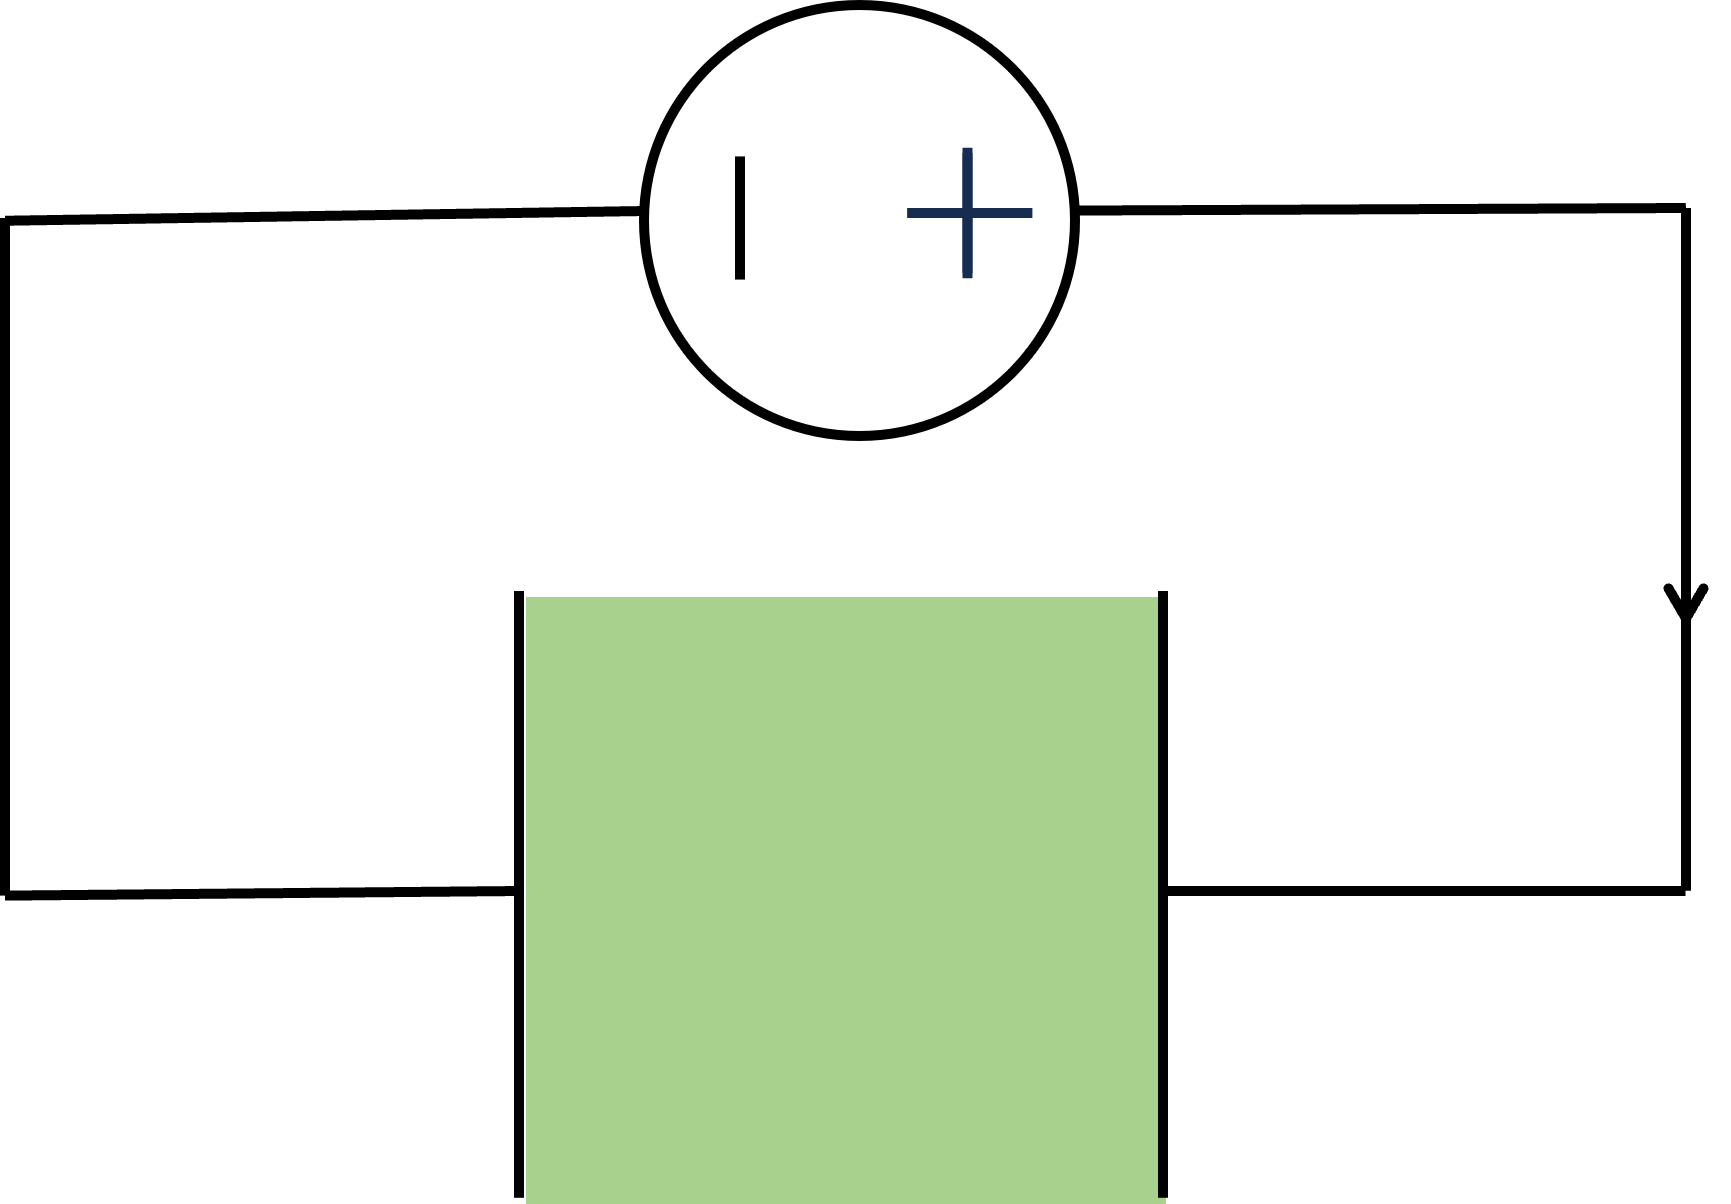
\includegraphics[width=0.4\textwidth]{pictures/circuit_dielectric.png}};
		\begin{scope}[x={(image.south east)},y={(image.north west)}]
			\node (total current) at (1.04,0.5) {{\large \(i_{tot}\)}};
		\end{scope}
	\end{tikzpicture}
	\caption{Simple circuit with dielectric material used as a medium in a capacitor.}
	\label{fig:circuit}
\end{figure}

Consider a the ideal circuit in figure \ref{fig:circuit}, where the a dielectric material is used as a medium in the capacitor. Ampère-Maxwell law guarantees that the current in the circuit \(i_{tot}\) is equivalent to the sum of conduction and displacement currents through the dielectric.
\subsection{Conduction current}
To compute conduction current entering in the dielectric from an electrode, we estimate the voltage gradient at its interface, say \(\Gamma_{c}\). In particular:
\begin{equation}\label{eq:cond-current1}
	I_c = \int_{\Gamma_{c}} \sigma \nabla \varphi \cdot \mathbf{n} \mathrm{d}\gamma
\end{equation}
We could, at this point, numerically integrate the expression in \eqref{eq:cond-current1}, estimating \(\nabla\varphi\) near the interface. However, it is also possible to turn \eqref{eq:cond-current1} into a volume integral and use the already available system matrix to compute it with a simple matrix-vector product. This is related with the core idea of Nanz method \cite{Nanz}.\\
Basically, given a test function \(u\), we have:
\begin{equation}\label{eq:cond-current2}
	\int_{\Gamma_{c}} \sigma \nabla \varphi \cdot \mathbf{n}\, u\, \mathrm{d}\gamma =
	\int_{\Omega} \sigma \nabla \varphi \cdot \nabla u\,\mathrm{d}\Omega +
	\int_{\Omega} \nabla \cdot \left( \sigma \nabla \varphi \right)\,u\,\mathrm{d}\Omega
\end{equation}
In a discrete contest we choose \(u = \sum_i \phi_i\) where \(\phi_i\) are the basis functions associated to the nodes on the electrode interface \(\Gamma_c\), so that the l.h.s. of \eqref{eq:cond-current2} is equivalent to \eqref{eq:cond-current1}. Noreover, with this choice of \(u\) volumetric integrals in \eqref{eq:cond-current2} are actually restricted to a thin strip near the electrode. If \(\varphi\) is regular enough and \(\sigma\) is constant in that strip, the second term in the r.h.s. of \eqref{eq:cond-current2} can be neglected. The first one, on the other hand, is associated to a stiffness matrix we can easily assemble. Once we know the solution for \(\varphi\), \(I_c\) can be computed with a simple matrix-vector product.
\subsection{Displacement current}
Displacement current can be deduced quantifying the variation of free charge on the interfaces of the conductors. This is also achieved through a matrix-vector product (this time with a mass matrix).

\section{Results}
For most of our tests we considered a cubic shaped domain with 1 mm edge. On the upper and lower sides a voltage (Dirichlet boundary conditions for \(\varphi\)) is imposed. On the upper the voltage is time dependent, while on the lower side it is fixed to 0. A charging transient is first simulated. Then, once the variables stabilize, we simulate a discharging transient.
\subsection{Test 1: Homogeneous material 1}
\begin{figure}
	\centering
	\begin{minipage}{0.5\textwidth}
		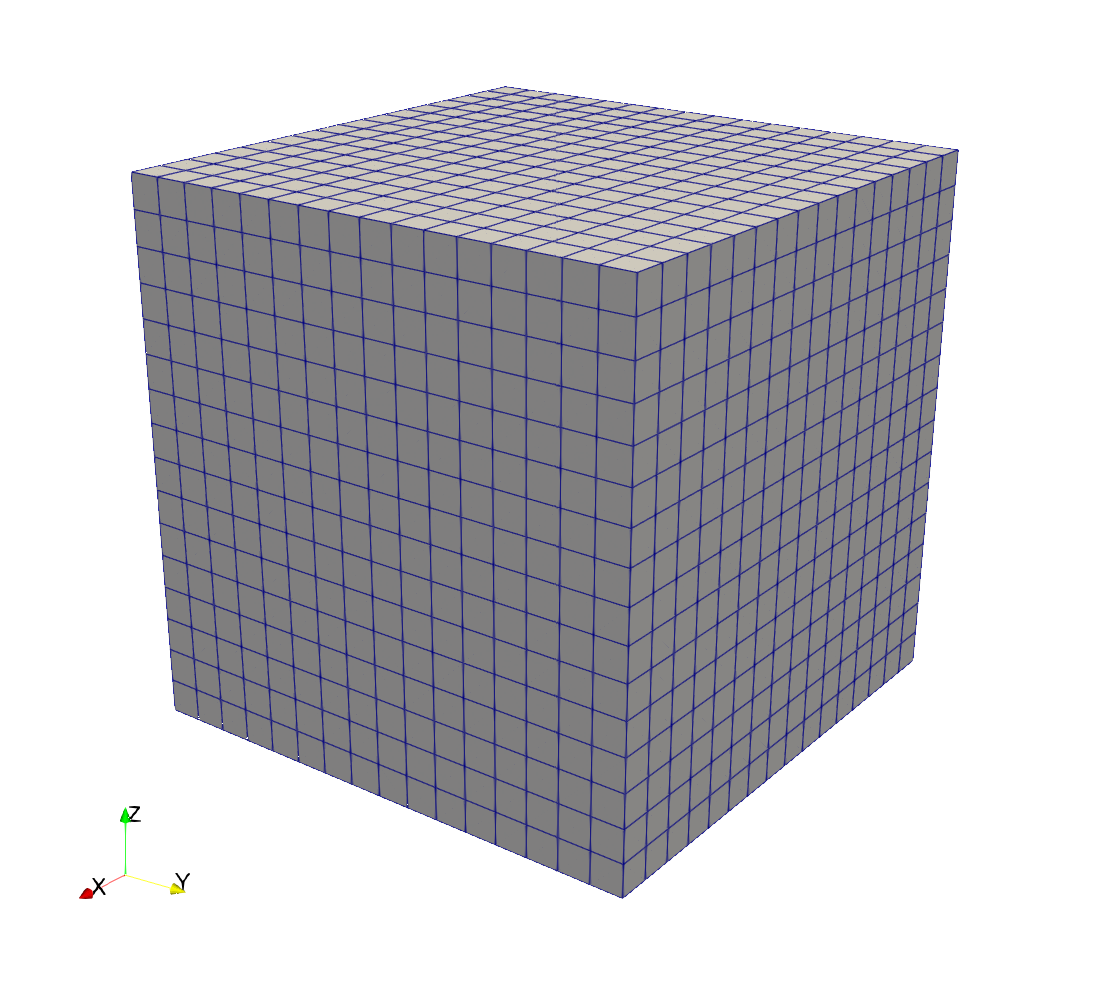
\includegraphics[width=\textwidth]{pictures/uniform-grid.png}
	\end{minipage}
	\begin{minipage}[t]{0.4\textwidth}
		\caption{Uniform grid}
		\label{fig:unif-grid}
	\end{minipage}
	\label{fig:geom-homog}
\end{figure}
\begin{figure}
	\subfloat[]{
		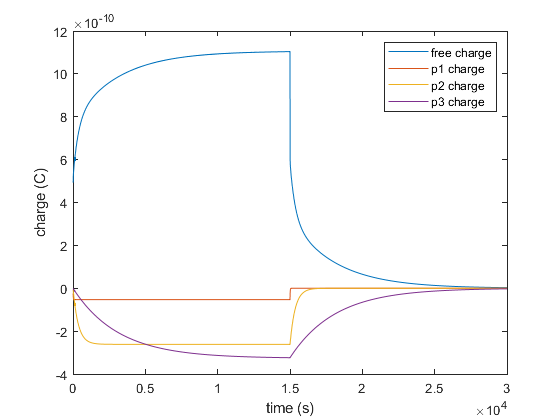
\includegraphics[width=0.54\textwidth]{pictures/test1_charges_on_c1.png}
	}
	\subfloat[]{
		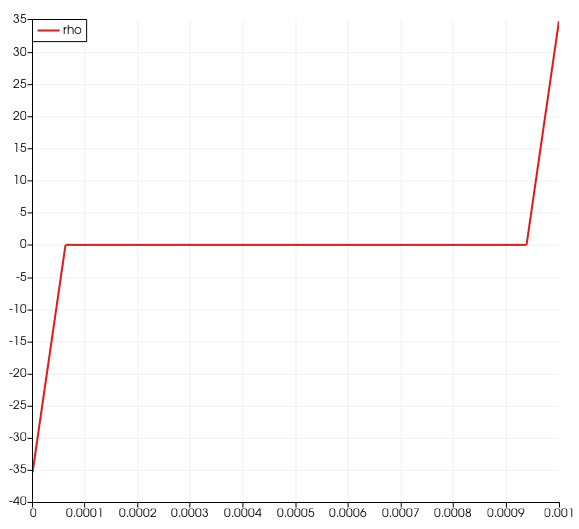
\includegraphics[width=0.44\textwidth]{pictures/test1_max_rho_profile.png}
	}\\
	\subfloat[]{
	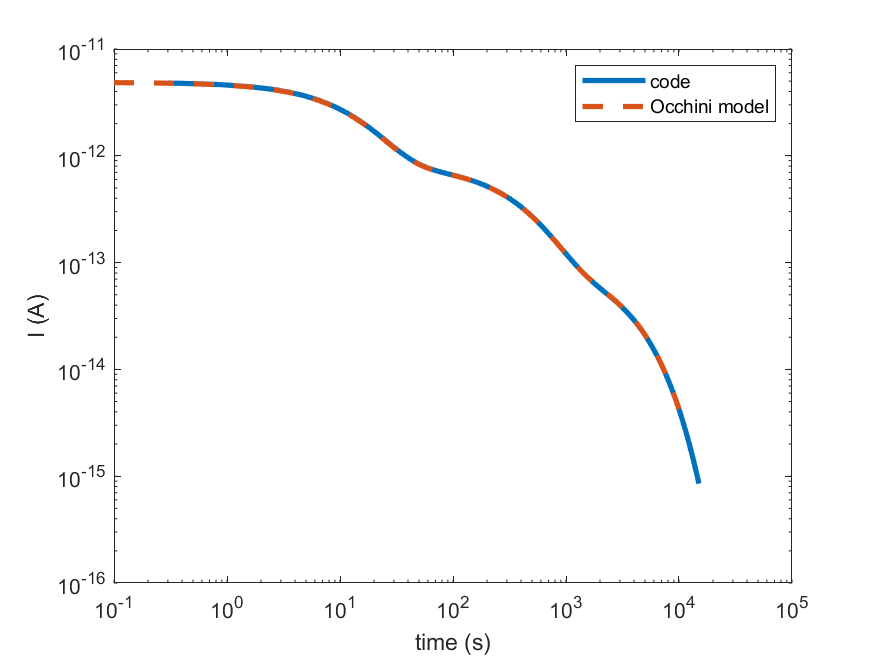
\includegraphics[width=0.54\textwidth]{pictures/codeVSocchini.png}
	}
	\subfloat[]{
	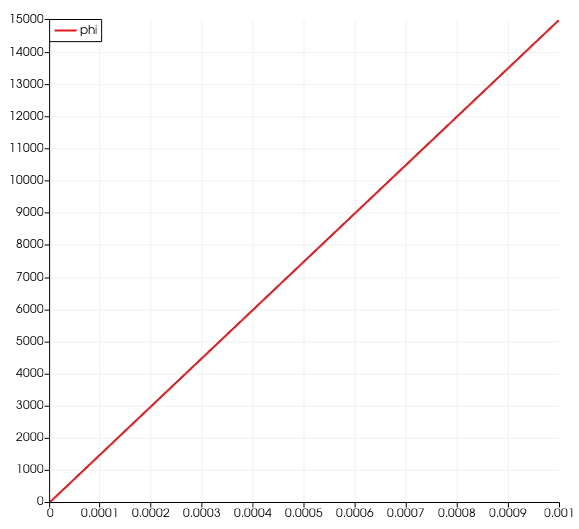
\includegraphics[width=0.44\textwidth]{pictures/test1_max_phi_profile.png}
	}
	\caption{Refinement procedure of a cell. On the left the uniform grid, on the right the grid refined in the cell 0.}
	\label{fig:octant_refinement}
	
\end{figure}
\subsection{Test 2: Homogeneous material 2}
\begin{figure}
	\subfloat[]{
		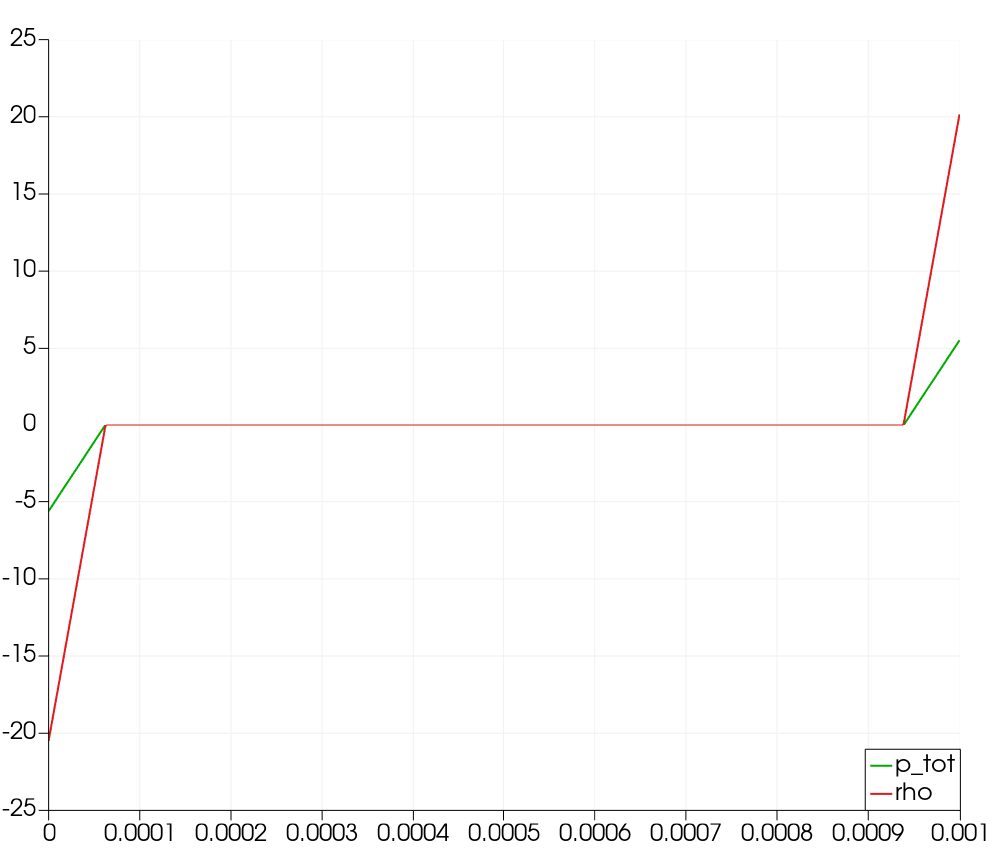
\includegraphics[width=0.5\textwidth]{pictures/homog1-pol-charges-on-z.png}
	}
	\subfloat[]{
		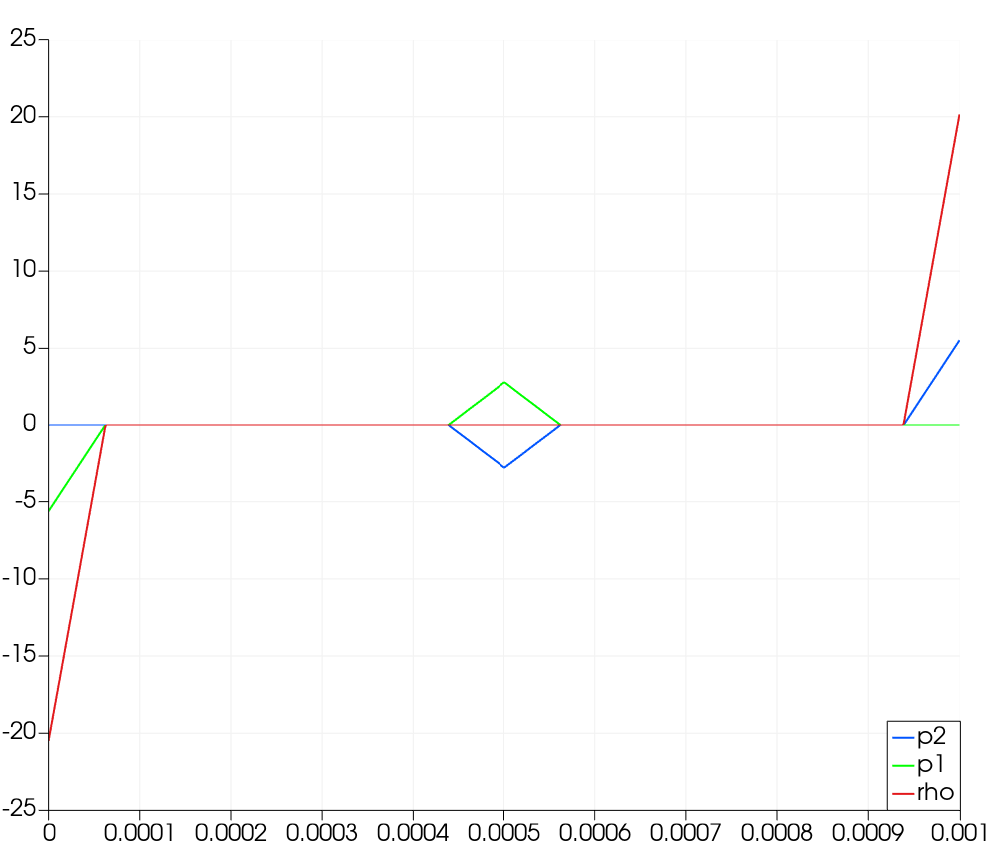
\includegraphics[width=0.5\textwidth]{pictures/homog2-pol-charges-on-z.png}
	}
	\caption{Refinement procedure of a cell. On the left the uniform grid, on the right the grid refined in the cell 0.}
	\label{fig:octant_refinement}
	
\end{figure}
\subsection{Test 3: Bi-phase material}
\subsection{Test 4: Homogeneous material with hole}
\subsection{Test 5: Butt gap}

%-----------------------------------------------------------------------------
% EQUATIONS
%-----------------------------------------------------------------------------
\begin{comment}\section{Equations}
\label{sec:eqs}
This section gives some examples of writing mathematical equations in your thesis.

Maxwell's equations read:
\begin{subequations}
    \label{eq:maxwell}
    \begin{align}[left=\empheqlbrace]
    \nabla\cdot \bm{D} & = \rho, \label{eq:maxwell1} \\
    \nabla \times \bm{E} +  \frac{\partial \bm{B}}{\partial t} & = \bm{0}, \label{eq:maxwell2} \\
    \nabla\cdot \bm{B} & = 0, \label{eq:maxwell3} \\
    \nabla \times \bm{H} - \frac{\partial \bm{D}}{\partial t} &= \bm{J}. \label{eq:maxwell4}
    \end{align}
\end{subequations}

Equation~\eqref{eq:maxwell} is automatically labeled by \texttt{cleveref},
as well as Equation~\eqref{eq:maxwell1} and Equation~\eqref{eq:maxwell3}.
Thanks to the \verb|cleveref| package, there is no need to use \verb|\eqref|.
Equations have to be numbered only if they are referenced in the text.

Equations~\eqref{eq:maxwell_multilabels1}, \eqref{eq:maxwell_multilabels2}, \eqref{eq:maxwell_multilabels3}, and \eqref{eq:maxwell_multilabels4} show again Maxwell's equations without brace:
\begin{align}
    \nabla\cdot \bm{D} & = \rho, \label{eq:maxwell_multilabels1} \\
    \nabla \times \bm{E} +  \frac{\partial \bm{B}}{\partial t} &= \bm{0}, \label{eq:maxwell_multilabels2} \\
    \nabla\cdot \bm{B} & = 0, \label{eq:maxwell_multilabels3} \\
    \nabla \times \bm{H} - \frac{\partial \bm{D}}{\partial t} &= \bm{J} \label{eq:maxwell_multilabels4}.
\end{align}

Equation~\eqref{eq:maxwell_singlelabel} is the same as before,
but with just one label:
\begin{equation}
    \label{eq:maxwell_singlelabel}
    \left\{
    \begin{aligned}
    \nabla\cdot \bm{D} & = \rho, \\
    \nabla \times \bm{E} +  \frac{\partial \bm{B}}{\partial t} &= \bm{0},\\
    \nabla\cdot \bm{B} & = 0, \\
    \nabla \times \bm{H} - \frac{\partial \bm{D}}{\partial t} &= \bm{J}.
    \end{aligned}
    \right.
\end{equation}

%-----------------------------------------------------------------------------
% FIGURES, TABLES AND ALGORITHMS
%-----------------------------------------------------------------------------
\section{Figures, Tables and Algorithms}

Figures, Tables and Algorithms have to contain a Caption that describes their content, and have to be properly referred in the text.

\subsection{Figures}
\label{subsec:figures}

For including pictures in your text you can use \texttt{TikZ} for high-quality hand-made figures \cite{tikz},
or just include them with the command
\begin{verbatim}
\includegraphics[options]{filename.xxx}
\end{verbatim}
Here xxx is the correct format, e.g.  \verb|.png|, \verb|.jpg|, \verb|.eps|, \dots.

\begin{figure}[H]
    \centering
    
\includegraphics[width=0.3\textwidth]{logo_polimi_scritta.eps}
    \caption{Caption of the Figure.}
    \label{fig:quadtree}
\end{figure}

Thanks to the \texttt{\textbackslash subfloat} command, a single figure, such as Figure~\ref{fig:quadtree},
can contain multiple sub-figures with their own caption and label, e.g. Figure~\ref{fig:polimi_logo1} and Figure~\ref{fig:polimi_logo2}. 

\begin{figure}[H]
    \centering
    \subfloat[One PoliMi logo.\label{fig:polimi_logo1}]{
        
\includegraphics[scale=0.5]{Images/logo_polimi_scritta.eps}
    }
    \quad
    \subfloat[Another one PoliMi logo.\label{fig:polimi_logo2}]{
        
\includegraphics[scale=0.5]{Images/logo_polimi_scritta2.eps}
    }
    \caption[]{Caption of the Figure.}
    \label{fig:quadtree2}
\end{figure}

\subsection{Tables}
\label{subsec:tables}

Within the environments \texttt{table} and  \texttt{tabular} you can create very fancy tables as the one shown in Table~\ref{table:example}.

\begin{table}[H]
    \caption*{\textbf{Example of Table (optional)}}
    \centering 
    \begin{tabular}{|p{3em} c c c |}
    \hline
    \rowcolor{bluePoli!40}
     & \textbf{column1} & \textbf{column2} & \textbf{column3} \T\B \\
    \hline \hline
    \textbf{row1} & 1 & 2 & 3 \T\B \\
    \textbf{row2} & $\alpha$ & $\beta$ & $\gamma$ \T\B\\
    \textbf{row3} & alpha & beta & gamma \B\\
    \hline
    \end{tabular}
    \\[10pt]
    \caption{Caption of the Table.}
    \label{table:example}
\end{table}

You can also consider to highlight selected columns or rows in order to make tables more readable.
Moreover, with the use of \texttt{table*} and the option \texttt{bp} it is possible to align them at the bottom of the page. One example is presented in Table~\ref{table:exampleC}. 

\begin{table*}[bp]
\centering 
    \begin{tabular}{|p{3em} | c | c | c | c | c | c|}
    \hline
%    \rowcolor{bluePoli!40}
     & \textbf{column1} & \textbf{column2} & \textbf{column3} & \textbf{column4} & \textbf{column5} & \textbf{column6} \T\B \\
    \hline \hline
    \textbf{row1} & 1 & 2 & 3 & 4 & 5 & 6 \T\B\\
    \textbf{row2} & a & b & c & d & e & f \T\B\\
    \textbf{row3} & $\alpha$ & $\beta$ & $\gamma$ & $\delta$ & $\phi$ & $\omega$ \T\B\\
    \textbf{row4} & alpha & beta & gamma & delta & phi & omega \B\\
    \hline
    \end{tabular}
    \\[10pt]
    \caption{Highlighting the columns}
    \label{table:exampleC}
\end{table*}

\subsection{Algorithms}
\label{subsec:algorithms}

Pseudo-algorithms can be written in \LaTeX{} with the \texttt{algorithm} and \texttt{algorithmic} packages.
An example is shown in Algorithm~\ref{alg:var}.
\begin{algorithm}[H]
\label{alg:example}
\caption{Name of the Algorithm}
\label{alg:var}
\label{protocol1}
\begin{algorithmic}[1]
\STATE Initial instructions
\FOR{$for-condition$}
\STATE{Some instructions}
\IF{$if-condition$}
\STATE{Some other instructions}
\ENDIF
\ENDFOR
\WHILE{$while-condition$}
\STATE{Some further instructions}
\ENDWHILE
\STATE Final instructions
\end{algorithmic}
\end{algorithm} 

\section{Some further useful suggestions}

Theorems have to be formatted as follows:
\begin{theorem}
\label{a_theorem}
Write here your theorem. 
\end{theorem}
\textit{Proof.} If useful you can report here the proof.
\vspace{0.3cm} % Insert vertical space

Propositions have to be formatted as follows:
\begin{proposition}
Write here your proposition.
\end{proposition}
\vspace{0.3cm} % Insert vertical space

How to insert itemized lists:
\begin{itemize}
    \item first item;
    \item second item.
\end{itemize}
How to write numbered lists:
\begin{enumerate}
    \item first item;
    \item second item.
\end{enumerate}

\section{Use of copyrighted material}

Each student is responsible for obtaining copyright permissions, if necessary, to include published material in the thesis.
This applies typically to third-party material published by someone else.

\section{Plagiarism}

You have to be sure to respect the rules on Copyright and avoid an involuntary plagiarism.
It is allowed to take other persons' ideas only if the author and his original work are clearly mentioned.
As stated in the Code of Ethics and Conduct, Politecnico di Milano \textit{promotes the integrity of research,
condemns manipulation and the infringement of intellectual property}, and gives opportunity to all those
who carry out research activities to have an adequate training on ethical conduct and integrity while doing research.
To be sure to respect the copyright rules, read the guides on Copyright legislation and citation styles available
at:
\begin{verbatim}
https://www.biblio.polimi.it/en/tools/courses-and-tutorials
\end{verbatim}
You can also attend the courses which are periodically organized on "Bibliographic citations and bibliography management".

%-----------------------------------------------------------------------------
% CONCLUSION
%-----------------------------------------------------------------------------
\section{Conclusions}
\color{black}
A final section containing the main conclusions of your research/study
and possible future developments of your work have to be inserted in the section ``Conclusions''.

\section{Bibliography and citations}
Your thesis must contain a suitable Bibliography which lists all the sources consulted on developing the work.
The list of references is placed at the end of the manuscript after the chapter containing the conclusions.
It is suggested to use the BibTeX package and save the bibliographic references in the file \verb|bibliography.bib|.
This is indeed a database containing all the information about the references. To cite in your manuscript, use the \verb|\cite{}| command as follows:
\\
\textit{Here is how you cite bibliography entries: \cite{knuth74}, or multiple ones at once: \cite{knuth92,lamport94}}.
\\
The bibliography and list of references are generated automatically by running BibTeX \cite{bibtex}.
\end{comment}
%-----------------------------------------------------------------------------
% BIBLIOGRAPHY
%-----------------------------------------------------------------------------
\bibliography{bibliography.bib}
\begin{comment}
\appendix
\section{Appendix A}
If you need to include an appendix to support the research in your thesis, you can place it at the end of the manuscript.
An appendix contains supplementary material (figures, tables, data, codes, mathematical proofs, surveys, \dots)
which supplement the main results contained in the previous sections.

\section{Appendix B}
It may be necessary to include another appendix to better organize the presentation of supplementary material.
\end{comment}
%%%%%%%%%%%%%%%%%%%%%%%%%%%%%%%%%%%%%%%%%%%%%%%%%%%%%%%%%%%%%%
%%     ABSTRACT IN ITALIAN LANGUAGE AND ACKNOWLEDGMENTS     %%
%%%%%%%%%%%%%%%%%%%%%%%%%%%%%%%%%%%%%%%%%%%%%%%%%%%%%%%%%%%%%%
\cleardoublepage

%-----------------------------------------------------------------------------
% SOMMARIO
%-----------------------------------------------------------------------------
\section*{Abstract in lingua italiana}
Qui va l'Abstract in lingua italiana della tesi seguito dalla lista di parole chiave.
\vspace{15pt}
\begin{tcolorbox}[arc=0pt, boxrule=0pt, colback=bluePoli!60, width=\textwidth, colupper=white]
    \textbf{Parole chiave:} qui, le parole chiave, della tesi, in italiano 
\end{tcolorbox}

%-----------------------------------------------------------------------------
% ACKNOWLEDGEMENTS
%-----------------------------------------------------------------------------
\section*{Acknowledgements}
Here you might want to acknowledge someone.

%-------------------------------------------------------------------------
%	END OF YOUR DOCUMENT
%-------------------------------------------------------------------------
\end{document}